\documentclass[12pt,a4paper]{report}
\usepackage{vntex}
\usepackage{extsizes}
%\usepackage[english,vietnam]{babel}
%\usepackage[utf8]{inputenc}

\usepackage[utf8]{inputenc}
%\usepackage[francais]{babel}
\usepackage{a4wide,amssymb,epsfig,latexsym,array,hhline,fancyhdr}
\usepackage{float}
\usepackage{amsmath}
\usepackage{amsthm}
\usepackage{multicol,longtable,amscd}
\usepackage{diagbox}%Make diagonal lines in tables
\usepackage{booktabs}
\usepackage{alltt}
\usepackage[framemethod=tikz]{mdframed}% For highlighting paragraph backgrounds
\usepackage{caption,subcaption}
\usepackage{logicproof}
\usepackage{lastpage}
\usepackage[lined,boxed,commentsnumbered]{algorithm2e}
\usepackage{enumerate}
\usepackage{color}
\usepackage{graphicx}							% Standard graphics package
\usepackage{array}
\usepackage{tabularx, caption}
\usepackage{multirow}
\usepackage{multicol}
\usepackage{rotating}
\usepackage{graphics}
\usepackage{geometry}
\geometry{%?i?u ch?nh gi?y cho c? file
    a4paper,%Gi?y A4
    total={170mm,257mm},%C? gi?y
    left=15mm,%L? tr?i
    right=15mm,%L? ph?i
    top=15mm,%L? tr?n
    bottom=15mm,%L? d??i
}
\usepackage{setspace}
\usepackage{epsfig}
\usepackage{tikz,tikz-timing}
\usetikzlibrary{arrows, shapes, calc}
\tikzstyle{decision} = [diamond, draw,
text width=3.5cm, text centered, inner sep=0pt]
\tikzstyle{block} = [rectangle, draw,
text width=5em, text centered, rounded corners, minimum height=4em]
\tikzstyle{arrow} = [draw, -latex']
\tikzstyle{round} = [circle, draw, inner sep=0pt, minimum size=2cm]
\tikzstyle{cloud} = [draw, ellipse, minimum height=2em]
\tikzstyle{input} =[trapezium, trapezium left angle=70, trapezium right angle=110, minimum width=3cm, minimum height=1cm, text centered, draw]
\tikzstyle{branch}=[fill, shape=circle, minimum size=3pt, inner sep=0pt]
\def\degr{${}^\circ$}
\usepackage[unicode]{hyperref}
\hypersetup{urlcolor=blue,linkcolor=black,citecolor=black,colorlinks=true}

\begin{document}
    \begin{titlepage}
        \begin{center}
            {\scshape\large ĐẠI HỌC QUỐC GIA THÀNH PHỐ HỒ CHÍ MINH\par}
                    {\scshape\LARGE TRƯỜNG ĐẠI HỌC BÁCH KHOA\par}
            {\scshape\Large KHOA KHOA HỌC - KỸ THUẬT MÁY TÍNH}
            \vspace{2cm}

        \end{center}
        \begin{figure}[H]
            \centering
            
\includegraphics[scale=.2]{LogoBK.jpg}
        \end{figure}
        \vspace{2cm}
        \begin{center}
            {\scshape \LARGE \textbf{Bộ môn Kỹ thuật lập trình}\par}
            \vspace{1cm}
            \Large \textbf{Báo cáo Bài tập lớn số 2: Chương trình quản lý thư viện LIBPRO}
        \end{center}
        \vspace{2cm}
        \begin{center}
            \begin{tabular}{r l}
                GVHD:&TS. Lê Thành Sách\\
                Sinh viên:&Nguyễn Anh Khoa - 1611617\\
                &Nguyễn Minh Khôi - 1611657\\
                &Phạm Quốc Nam - 1612128\\
            VSTS:& \url{https://thaoxkhoa.visualstudio.com/_git/LIBPRO}\\
            &(VSTS là một dịch vụ private, chỉ những thành viên mới được phép truy cập)\\
            Github:& \url{https://github.com/nganhkhoa/LIBRPO}\\
            &(github là được chuyển lại từ VSTS, nên không có lịch sử đầy đủ)
            \end{tabular}\\
        \end{center}
    \end{titlepage}
\newpage
\chapter{Tổng quan về LIBPRO}
LIBPRO. được sự gợi ý và thúc đẩy của các Giảng viên Môn Kỹ Thuật Lập Trình, là một phần mềm chuyên biệt quản trị các hoạt động trong các thư viện thông thường. LIBPRO tuy chưa phải phần mềm hoàn hảo nhất về các tiện ích và giao diện người dùng, nhưng đã đáp ứng được các yêu cầu cơ bản cho những người sử dụng. LIBPRO là sản phẩm của SIMple Group, gồm các thành viên Nguyễn Anh Khoa, Nguyễn Minh Khôi và Phạm Quốc Nam cùng phát triển.
\chapter{Phần mềm Quản lý Thư viện LIBPRO}
    \section{Đôi nét cơ bản về LIBPRO}
    LIBPRO là chương trình quản lý thư viện được xây dựng trên nền tảng ngôn ngữ C++ kết hợp với GUI Qt..., lưu dữ liệu người dùng, sách và yêu cầu mượn ỏ dạng file .json. LIBPRO được phát triển nhằm mục đích nghiên cứu và rèn luyện, nhiều tính năng mở rộng vẫn chưa được hoàn thiện, chỉ mới ở mặt ý tưởng.
    \section{Hướng dẫn cài đặt phần mềm}
    \section{Hướng dẫn sử dụng phần mềm}
        \subsection{Đăng nhập}
            \subsection{Đăng ký}
            Khi chưa có hồ sơ người dùng LIBPRO, chọn \textbf{Profile->Log In} và chọn vào ô chưa đăng ký để đăng ký.\\
            Các thông tin yêu cầu bắt buộc khi đăng ký là họ và tên người đăng ký, tên người dùng trong LIBPRO và số CMND (hoặc số thẻ căn cước).\\
            Sau khi đăng ký, người dùng sẽ được tạo một mật khẩu mới bất kỳ để đăng nhập vào LIBPRO, sau đó người dùng có thể chỉnh sửa lại mật khẩu.\\
            \subsection{Đăng nhập}
            Khi đã có hồ sơ người dùng LIBPRO, chọn \textbf{Profile->Log In} và nhập tên người dùng LIBPRO và mật khẩu để đăng nhập.\\
            Nếu quên mật khẩu, hãy nhấn vào ô tạo mật khẩu mới, và lúc này, hồ sơ người dùng sẽ được khóa lại, chờ khi người dùng nhận được mật khẩu mới từ QUẢN LÝ NGƯỜI DÙNG.\\
            \subsection{Đăng xuất}
            Nếu đã hoàn thành công việc trên hồ sơ của mình, người dùng có thể đăng xuất bằng cách chọn trên thanh menu \textbf{Profile->Log Out}.\\
            \subsection{Tùy chỉnh khác}
            Tạo mới tài khoản : các chức năng trong thư viện được cấp phát thông qua tài khoản của người dùng, vì vậy cần thiết tạo tài khoản cho người dùng bằng cách: trên thanh menu, chọn \textbf{Profile->New Account}.\\
            Để chuyển đổi giữa các tài khoản, chọn trên thanh menu \textbf{Profile->Choose Account}.\\
            Để chỉnh sửa các thông tin người dùng, bao gồm cả tên tài khoản, và mật khẩu người dùng, chọn \textbf{Profile->Edit->...} tùy theo nhu cầu của người dùng.\\
        \subsection{Xem thông báo}
            Có hai mục để xem là xem theo lịch sử và xem theo các thông báo chưa xem bao giờ.\\
        \subsection{Tùy chỉnh}
            \subsubsection{Chủ đề của LIBPRO} (tính năng mở rộng chưa được cập nhật)\\
            \subsubsection{Ngôn ngữ của LIBRPO} (tính năng mở rộng chưa được cập nhật)\\
        \subsection{Duyệt sách}
        Trên thanh menu, chọn \textbf{Library->View All Book} để xem toàn bộ sách trong thư viện.\\
        Nếu muốn tìm sách, chọn \textbf{Library->View All Book} và nhập tên sách người dùng muốn tìm vào thanh Search và chọn \textbf{Find} để tìm sách.\\
            \subsubsection{Sách yêu thích}
            Nếu muốn thêm sách vào mục yêu thích, chọn \textbf{Library->View All Book} và chọn \textbf{Add to Favorites} tại quyển sách mà người dùng thích.\\
            Để xem các sách yêu thích đã chọn, trên thanh menu, chọn \textbf{Library->Favorites}.\\
            Nếu không thích quyển sách nào trong mục yêu thích, người dùng nhấp vào nút \textbf{Out Favorites} để xóa sách đó khỏi mục yêu thích.\\
            \subsubsection{Mượn sách}
            Tại màn hình duyệt sách hoặc màn hình mục yêu thích hoặc màn hình tìm sách, nhấp vào nút \textbf{Add to Cart} để thêm sách vào giỏ.\\
            Nếu người dùng đã có tài khoản với chức năng READER, trên thanh menu, chọn \textbf{Role->READER->Cart} để gửi yêu cầu mượn sách đến thủ thư và chờ sự xác nhận của thủ thư.\\
        \subsection{Chức năng}
            Chọn trên thanh menu, \textbf{Role}, và lựa chọn các chức năng bên dưới. Lưu ý là chỉ những chức năng của tài khoản hiện thời mới khả dụng.\\
            \subsubsection{READER - ĐỘC GIẢ}
            \begin{enumerate}
                \item xem giở hàng: vào \textbf{READER->Cart} để xem giỏ hàng của người dùng, để đăng ký mượn sách.
                \item Photocopy: có thể photo các sách cho phép photo (tính năng mở rộng chưa được cập nhật)
            \end{enumerate}
            \subsubsection{REVIEWER - NHÀ PHÊ BÌNH}
            Có thể thêm review vào sách, (tính năng mở rộng chưa được cập nhật)\\
            \subsubsection{CD - XEM SÁCH NÓI}
            Có thể duyệt vào các sách nói, (tính năng mở rộng chưa được cập nhật)\\
            \subsubsection{MOVIE - XEM PHIM TƯ LIỆU}
            Có thể duyệt các phim tư liệu, các video học thuật, (tính năng mở rộng chưa được cập nhật)\\
            \subsubsection{EBOOK - NHÀ PHÊ BÌNH}
            Có thể duyệt các sách điện tử, (tính năng mở rộng chưa được cập nhật)\\
            \subsubsection{VIP}
            Có thể duyệt tất cả các loại sách, tư liệu và phê bình, (tính năng mở rộng chưa được cập nhật)\\
            \subsubsection{LIBRARIAN - THỦ THƯ}
                \begin{enumerate}
                    \item Duyệt yêu cầu mượn sách: vào \textbf{Role->LIBRARIAN->Browse Borrow} để duyệt các yêu cầu mượn sách từ người dùng.
                    \item Quản lý sách: vào \textbf{Role->LIBRARIAN->Book Management} để thêm sách, xóa sách và thay đổi các thông tin của sách.
                \end{enumerate}
            \subsubsection{USER ADMINISTRATOR - QUẢN LÝ NGƯỜI DÙNG}
                \begin{enumerate}
                    \item Quản lý hồ sơ người dùng: vào \textbf{Role->USER ADMINISTRATOR->Profile Management} để thêm, xóa người dùng và tạo mật khẩu mới cho người dùng quên mật khẩu.
                    \item Thêm vào danh sách đặc biệt : (tính năng mở rộng chưa được cập nhật).
                    \item Khóa hồ sơ người dùng: \textbf{Role->USER ADMINISTRATOR->Lock} để khóa các hồ sơ vi phạm.
                \end{enumerate}
            \subsubsection{ACCOUNTANT - QUẢN LÝ TÀI CHÍNH}
            Quản lý chi tiêu của thư viện và của người dùng. (tính năng mở rộng chưa được cập nhật)
        \subsection{Trợ giúp}
            \begin{enumerate}
                \item Đọc hướng dẫn sử dụng thư viện.
                \item Đọc hướng dẫn sử dụng LIBPRO.
                \item Về người phát triển phần mềm.
                \item Liên hệ.
            \end{enumerate}
\chapter{Tiến trình thực hiện phần mềm}
    \section{Phân tích hoạt động của thư viện}
        \subsection{Vai trò người sử dụng}
        LIBPRO cung cấp 4 vai trò chủ yếu cho người sử dụng:
        \begin{enumerate}
            \item KHÁCH
            \item ĐỘC GIẢ
            \item THỦ THƯ
            \item QUẢN LÝ NGƯỜI DÙNG
        \end{enumerate}
            \subsubsection{KHÁCH}
                KHÁCH được định nghĩa là người được truy cập vào phần mềm LIBPRO, tuy nhiên, KHÁCH chỉ có thể xem phần trợ giúp \textbf{Help} trê thanh Menu. Số lượng KHÁCH truy cập vào phần mềm là không giới hạn
            \subsubsection{ĐỘC GIẢ}
                ĐỘC GIẢ được định nghĩa là người được truy cập vào phần mềm LIBPRO, có thể xem sách, xem thông báo, gửi yêu cầu mượn sách đến thủ thư, điều chỉnh các thông tin cá nhân, giao diện LIBPRO.
                Số lượng ĐỘC GIẢ truy cập vào phần mềm là có giới hạn, tùy theo quy định của thư viện.
            \subsubsection{THỦ THƯ}
                THỦ THƯ được định nghĩa là người được truy cập vào phần mềm LIBPRO, có khả năng quản lý sách, quản lý việc mượn và trả sách, gửi thông báo về sách mới, sách được mượn đến người dùng.
                Số lượng THỦ THƯ truy cập vào phần mềm là rất ít, do QUẢN LÝ THƯ VIỆN cấp phát.
            \subsubsection{QUẢN LÝ NGƯỜI DÙNG}
                QUẢN LÝ NGƯỜI DÙNG được định nghĩa là người được truy cập vào phần mềm LIBPRO, có khả năng quản lý hồ sơ người dùng, thêm, khóa hoặc xóa người dùng, gửi thông báo đến người dùng các thông tin liên quan đến hồ sơ người dùng.
                Số lượng QUẢN LÝ NGƯỜI DÙNG truy cập vào phần mềm rất ít, do QUẢN LÝ THƯ VIỆN cấp phát.\\
        Ngoài ra, LIBRPO còn cung cấp thêm một số vai trò khác
        \begin{enumerate}
            \item NHÀ SƯU TẦM: có thể mua sách
            \item NHÀ PHÊ BÌNH: có thể bình luận và đánh giá sách
            \item SÁCH NÓI: truy cập vào kho sách nói
            \item TƯ LIỆU PHIM ẢNH: truy cập vào kho phim tư liệu
            \item SÁCH ĐIỆN TỬ: truy cập vào kho sách điện tử
            \item VIP: có thể xem tất cả các loại sách, tư liệu
            \item QUẢN LÝ TÀI CHÍNH: quản lý các chi tiêu của thư viện và người dùng
        \end{enumerate}
        \subsection{Cấp độ quản lý và thực thi}
            \subsubsection{Cấp Người dùng}
            Đây là cấp lớn nhất và khái quát nhất trong môi trường LIBPRO.\\
            Một số đặc điểm của cấp Người dùng:
            \begin{enumerate}
                \item Cấp người dùng sẽ được cấp phát cho người dùng sau khi QUẢN LÝ NGƯỜI DÙNG chấp thuận yêu cầu đăng ký của người dùng.
                \item Tên gọi cấp Người dùng là duy nhất và không trùng lặp, xét cả trường hợp chữ in và chữ thường
                \item Tên gọi cấp Người dùng có độ dài không quá 32 ký tự và không chứa các ký tự đặc biệt (về các ký tự đặc biệt, xem kỹ hơn ở mục...)
                \item Một tên Người dùng có thể đăng ký nhiều tài khoản phân biệt và không trùng lặp
                \item Cấp người dùng chỉ được xóa khi người dùng gửi yêu cầu đến QUẢN LÝ NGƯỜI DÙNG hoặc do người dùng vi phạm các quy định của thư viện ở mức nào đó trở lên.
            \end{enumerate}

            \subsubsection{Cấp Tài khoản}
            Đây là cấp thứ hai sau cấp Người dùng trong môi trường LIBPRO.\\
            Một số đặc điểm của cấp Tài khoản:
            \begin{enumerate}
                \item Cấp Tài khoản sẽ có thể cấp phát cho người dùng sau khi QUẢN LÝ NGƯỜI DÙNG chấp thuận yêu cầu đăng ký của người dùng.
                \item Tên gọi cấp Tài khoản là duy nhất và không trùng lặp, xét cả trường hợp chữ in và chữ thường
                \item Tên gọi cấp Tài khoản có độ dài không quá 32 ký tự và không chứa các ký tự đặc biệt (về các ký tự đặc biệt, xem kỹ hơn ở mục...)
                \item Một tên Tài khoản có thể đăng ký nhiều vai trò phân biệt và không trùng lặp
                \item Cấp Tài khoản sẽ bị khóa nếu tài khoản đó được liệt vào danh sách đen. (Chi tiết về danh sách đen, xem mục...)
                \item Cấp tài khoản chỉ được xóa khi người dùng gửi yêu cầu đến QUẢN LÝ NGƯỜI DÙNG hoặc do người dùng vi phạm các quy định của thư viện ở mức nào đó trở lên.
            \end{enumerate}
            \subsubsection{Cấp vai trò}
            Như đã giới thiệu ở phần 2.1.1 về các vai trò người dùng, phần này xin bổ sung thêm một số quy định
            \begin{enumerate}
                \item Số vai trò trong 1 tài khoản tối đa có thể là 3
                \item Mỗi vai trò đặc trưng cho khả năng khai thác thư viện của người dùng với từng mức phí khác nhau
                \item Trong cùng một tài khoản, không thể cùng lúc thao tác ở 2 vai trò khác nhau. BUỘC phải chuyển từ vai trò A sang vai trò B để thực hiện công việc của B chứ không thể thực hiên công việc của B khi đang ở vai trò A.
            \end{enumerate}
        \subsection{Thủ tục đăng ký và đăng nhập}
        Viêc truy cập vào LIBPRO hoàn toàn chưa cần đến việc đăng ký, như đã nêu ở trên, nhưng để nâng cao mức thao tác, người sử dùng cần đăng ký người dùng và tài khoản LIBPRO.\\
            \subsubsection{Về việc Đăng ký}
            Người dùng sẽ nhấp vào ô đăng ký để thực hiên yêu cầu đăng ký của mình. Thông tin cần điền vào sẽ có những mục bắt buộc và không bắt buộc. Sau khi điền xong, người dùng sẽ nhấn nút gửi và chờ duyệt từ QUẢN LÝ NGƯỜI DÙNG. Vì thành viên của thư viện chỉ có giới hạn, nên không phải mọi người đều đăng ký thành công.\\
            Việc đăng ký thường chỉ xảy ra khi muốn tạo thêm tài khoản mới cho cấp Người dùng hiện tại. Nếu muốn đăng ký cấp Người dùng mới, phải đăng xuất khỏi cấp người dùng hiện tại để đăng ký.\\
            Về thông tin cần phải đăng ký:
            \begin{enumerate}
                \item Tên User (Là tên để khai báo trong LIBPRO)
                \item Họ và Tên người dùng (Là tên trong khai sinh)
                \item Ngày tháng năm sinh
                \item Giới tính
                \item Quốc tịch
                \item Dân tộc
                \item Số chứng minh nhân dân
                \item CMND cấp ngày
                \item Địa chỉ hiện tại
                \item Số điện thoại
                \item Công việc
                \item Cơ quan làm việc
                \item Địa chỉ cơ quan
            \end{enumerate}
            \subsubsection{Về việc Đăng nhập}
            Người dùng sẽ nhấp vào ô đăng nhập để đăng nhập vào hồ sơ người dùng của mình. Khi đăng nhập, chỉ cần điền tên người dùng và password của người dùng đó. Sau khi đăng nhập, mọi tùy chỉnh trước lần đăng xuất cuối cùng đều sẽ được giữ nguyên.\\
            Khi người dùng muốn thoát chương trình, cần thực hiện bước đăng xuất trước khi thoát.\\
            Nếu người dùng không đăng xuất trước khi thoát khỏi chương trình, ở lần mở chương trình tiếp theo, chương trình sẽ hiện lên tên tài khoản chưa đăng xuất và yêu cầu nhập password để truy cập vào tài khoản; hoặc truy cập như là KHÁCH.\\
            \subsubsection{Về các ký tự đặc biệt}
            Phần này chủ yếu dành cho việc đăt tên người dùng hoặc tên tài khoản.\\
            Các ký hiệu đặc biệt là: $ ! @ \# \$ \% \textasciicircum{} \& * ( ) < > ? $ và dấu cách
        \subsection{Quản lý sách}
            \subsubsection{Các đặc tính của sách}
            Sách trong LIBPRO được quản lý dựa trên các thông tin sau:
            \begin{enumerate}
                \item Mã ISBN
                \item Tên Đầu sách
                \item Tên tác giả (một hoặc nhiều tác giả)
                \item Nhà xuất bản
                \item Thể loại (một hoặc nhiều thể loại)
                \item Năm xuất bản
                \item Nội dung chính
            \end{enumerate}
            Sách trong thư viện sẽ được quản lý trực tiếp qua mã sách (ISBN), mỗi cuốn sách có một mã sách riêng biệt và không trùng lặp.\\
            \textbf{Thể loại:} Các thể loại sách được phân ra như sau:
            \begin{itemize}
                \item Hội họa và Nhiếp ảnh
                \item Sách Audio
                \item Tự truyện và Hồi ký
                \item Sách trên CD
                \item Tài chính và Tiền tệ
                \item Lịch
                \item Trẻ em
                \item Kinh Thánh và Sách Kitô giáo
                \item Truyện tranh
                \item Công nghệ và Máy tính
                \item Ẩm thực
                \item Sở thích và...
                \item Deals in Books
                \item Giáo dục và Đào tạo
                \item Cơ khí và Vận tải
                \item Đồng tính
                \item Sức khỏe
                \item Lịch Sử
                \item Hài hước
                \item Luật
                \item Văn học
                \item Y học
                \item Phiêu lưu mạo hiểm
                \item Làm cha mẹ
                \item Chính trị và Khoa học xã hội
                \item Tham khảo
                \item Tôn giáo và Tín ngưỡng
                \item Lãng mạn
                \item Khoa học và Toán học
                \item Khoa học viễn tưởng
                \item Kỹ năng sống
                \item Thể thao và Hoạt động Ngoài trời
                \item Lứa tuổi thiếu niên
                \item Ôn luyện các kỳ thi
                \item Sách giáo khoa
                \item Du lịch và Khám phá
            \end{itemize}
            \subsubsection{Sắp xếp sách}
            Sách được sắp xếp theo các tiêu chí giảm dần tính ưu tiên sau:
            \begin{itemize}
                \item Theo Thời điểm xuất bản (ưu tiên sách xuất bản gần đây)
                \item Theo Bảng chữ cái (A-Z hoặc Z-A)
                \item Theo Tên tác giả
                \item Theo Thể loại sách
                \item Theo Nhà xuất bản
            \end{itemize}

            \subsubsection{Nhập sách}
            Việc nhập sách được diễn ra định kỳ hoặc không định kỳ. Định kỳ 3 tháng hoặc 6 tháng sẽ có đợt sách mới về; sách mới có thể là:
            \begin{itemize}
                \item Giống sách đã có trong thư viện, việc nhập sách mới làm tăng số lượng sách chỉ của đầu sách đó
                \item Là sách hoàn toàn mới chưa có trong thư viện, việc nhập sách mới làm tăng số lượng các đầu sách
            \end{itemize}
            Việc nhập sách mới được quản lý và thông qua bởi quyết định của thủ thư.\\
            Sau khi nhập sách mới về, thủ thư cần chủ động gửi thông báo đến các độc giả còn quyền người dùng.\\

            \subsubsection{Mượn sách}
                \begin{enumerate}
                \item \textbf{Ai có thể mượn sách}\\
                Chỉ cấp vai trò ĐỘC GIẢ có quyền gửi yêu cầu mượn sách.\\
                Việc xác nhận yêu cầu mượn sách từ ĐỘC GIẢ do THỦ THƯ xử lý.\\
                \item \textbf{Có thể mượn sách trong bao lâu}\\
                Theo quy định hiện hành và phổ thông, mỗi đầu sách chỉ được mượn nhiều nhất là 2 tuần, kể từ ngày ghi trên yêu cầu mượn sách.\\
                Nếu có nhu cầu gia hạn, cấp vai trò THỦ THƯ sẽ quyết định nếu có thể gia hạn, và chỉ được gia hạn thêm 1 tuần là tối đa.\\
                \item \textbf{Một lần mượn được bao nhiêu quyển sách}\\
                Một lần mượn (tại thời điểm bất kỳ của thời gian mượn) thì một ĐỘC GIẢ chỉ có thể mượn tối đa 4 đầu sách.\\
                Tránh việc mượn hơn 1 quyển của cùng 1 đầu sách.\\
                \end{enumerate}
            \subsubsection{Trả sách}
                \begin{enumerate}
                \item \textbf{Khi nào phải trả sách}\\
                    Việc trả sách được thực hiện thông qua hai quy định sau:
                    \begin{enumerate}
                        \item Bất kỳ quyển sách nào được mượn đều phải trả lại thư viện trong vòng 2 tuần kể từ ngày ghi trên yêu cầu mượn sách, hoặc trong vòng 3 tuần nếu được gia hạn.\\
                        \item Thư viện có yêu cầu trả sách trước thời hạn vì một số lý do cụ thể.
                    \end{enumerate}
                    Trường hợp ĐỘC GIẢ không trả sách cho thư viện theo hai quy định trên, sẽ có mức xử phạt tương ứng.\\
                \item \textbf{Tình trạng sách}\\
                    Tình trạng sách là một đại lượng có tính tương đối tùy thuộc vào quy định thư viện.\\
                    Nếu sách bị hư hại thì thủ thư có quyền phạt tiền người dùng, bằng cách thông báo và trừ tiền trong tài khoản của ngươi dùng.\\
                    Nếu làm mất sách, thì phải xử phạt theo quy định thư viện.\\
                \end{enumerate}
        \subsection{Quản lý người dùng}
        Việc quản lý người dùng được thực hiện thông qua vai trò QUẢN LÝ NGƯỜI DÙNG.\\
            \subsubsection{Tạo cấp Người dùng}
            Khi nhận được yêu cầu đăng ký hồ sơ người dùng LIBPRO, QUẢN LÝ NGƯỜI DÙNG sẽ quyết định chấp thuận yêu cầu đăng ký hay không.\\

            \subsubsection{Cập nhật tình trạng người dùng}
            Dựa theo lịch sử đăng nhập và đăng xuất của người dùng để đánh giá và xếp loại người dùng theo các tiêu chí (tính năng mở rộng chưa được cập nhật)\\ %phan nay suy nghi sau

            \subsubsection{Danh sách Đỏ}
            Các tài khoản vi phạm quy định thư viện từ mức 3 đến mức 1 sẽ được liệt kê vào một danh sách gọi là danh sách Đỏ.\\

            \subsubsection{Khóa tài khoản và Danh sách Đen}
            Việc khóa tài khoản được thực hiện theo yêu cầu từ THỦ THƯ khi tài khoản này vi phạm các quy định từ mức 4 trở xuống.\\
            Đồng thời, khi bị khóa lần đầu, các tài khoản đó sẽ được liệt kê trong một danh sách, gọi là Danh sách Đen.\\
            Sau một khoảng thời gian (tùy vào thái độ của người dùng tài khoản), tài khoản từng bị khóa sẽ được mở, nhưng tên tài khoản vẫn nằm trong danh sách Đen.\\
            Các tài khoản bị liệt vào danh sách Đen sẽ chịu một số hạn chế khi sử dụng thư viện.\\

            \subsubsection{Xóa tài khoản và Xóa người dùng}
            Các tài khoản vi phạm quy định thư viện từ mức 6 trở xuống sẽ bị xóa tài khoản cùng mọi thông tin về tài khoản đó, trừ danh sách Đỏ và danh sách Đen\\
            Các người dùng vi phạm quy định thư viện từ mức 8 trở xuống sẽ bị xóa tài khoản cùng mọi thông tin về tài khoản đó, trừ danh sách Đỏ và danh sách Đen.\\
        %TÍNH NĂNG BỔ SUNG
        %tạo forum hoặc fanpage
        %hiện ra các sách liên quan đến sở thích người dùng, dùng thuật toán thống kê phân tích để xuất kết quả
    \newpage
    \section{Vẽ sơ đồ thiết kế dữ liệu}
        \subsection{Sơ đồ quản lý hồ sơ người dùng}
        Hồ sơ người dùng được chia ra 4 tập tin:
        \begin{enumerate}
            \item Tập tin chính quản lý người dùng
%
%            \begin{figure}[H]
%                \centering
%
%                \label{F:userfocus}
%                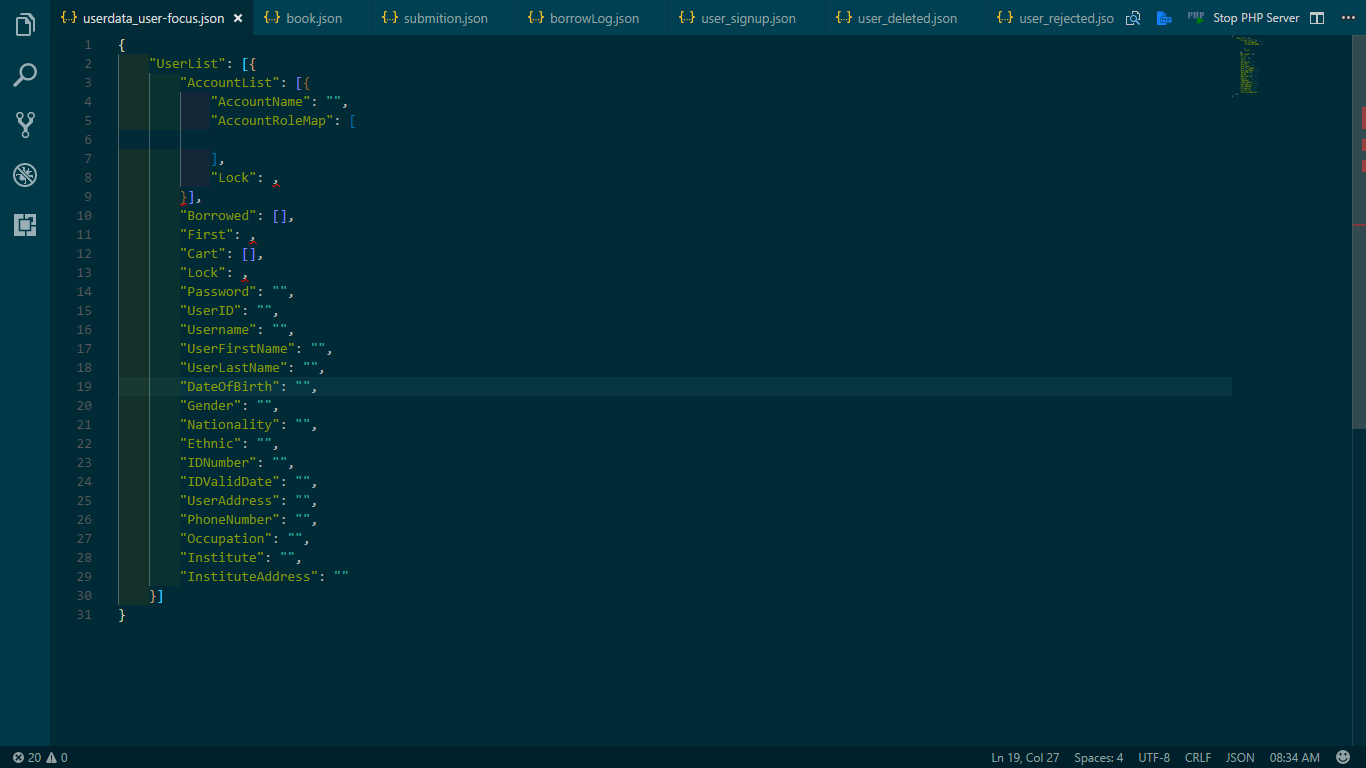
\includegraphics[scale = .3]{userfocus.png}
%                \caption{Sơ đồ các thuộc tính quản lý người dùng}
%            \end{figure}
%
            \begin{verbatim}
            {
                "UserList": [
                    {
                        "AccountList": [
                            {
                                "AccountName": string,
                                "AccountRoleMap": [
                                    numbers
                                ],
                                "Lock": bool
                            }
                        ],
                        "Balance": number double,
                        "Borrowed": [
                            {
                                "Submit ID": number,
                                "ISBN": string
                            }
                        ],
                        "Cart": [
                            strings
                        ],
                        "DateOfBirth": string,
                        "Ethnic":string,
                        "First": bool,
                        "Gender":string,
                        "IDNumber": string,
                        "IDValidDate": string,
                        "Institue": string,
                        "InstitueAddress": string,
                        "Nationality": string,
                        "Occupation": string,
                        "Password": string,
                        "PhoneNumber": string,
                        "UserAddress": string,
                        "UserFirstName": string,
                        "UserID": string,
                        "UserLastName": string,
                        "Username": string
                    }
                ]
            }
            \end{verbatim}
            \newpage
            \item Tập tin quản lý việc đăng ký
%            \begin{figure}[H]
%                \centering
%
%                \label{F:usersignup}
%                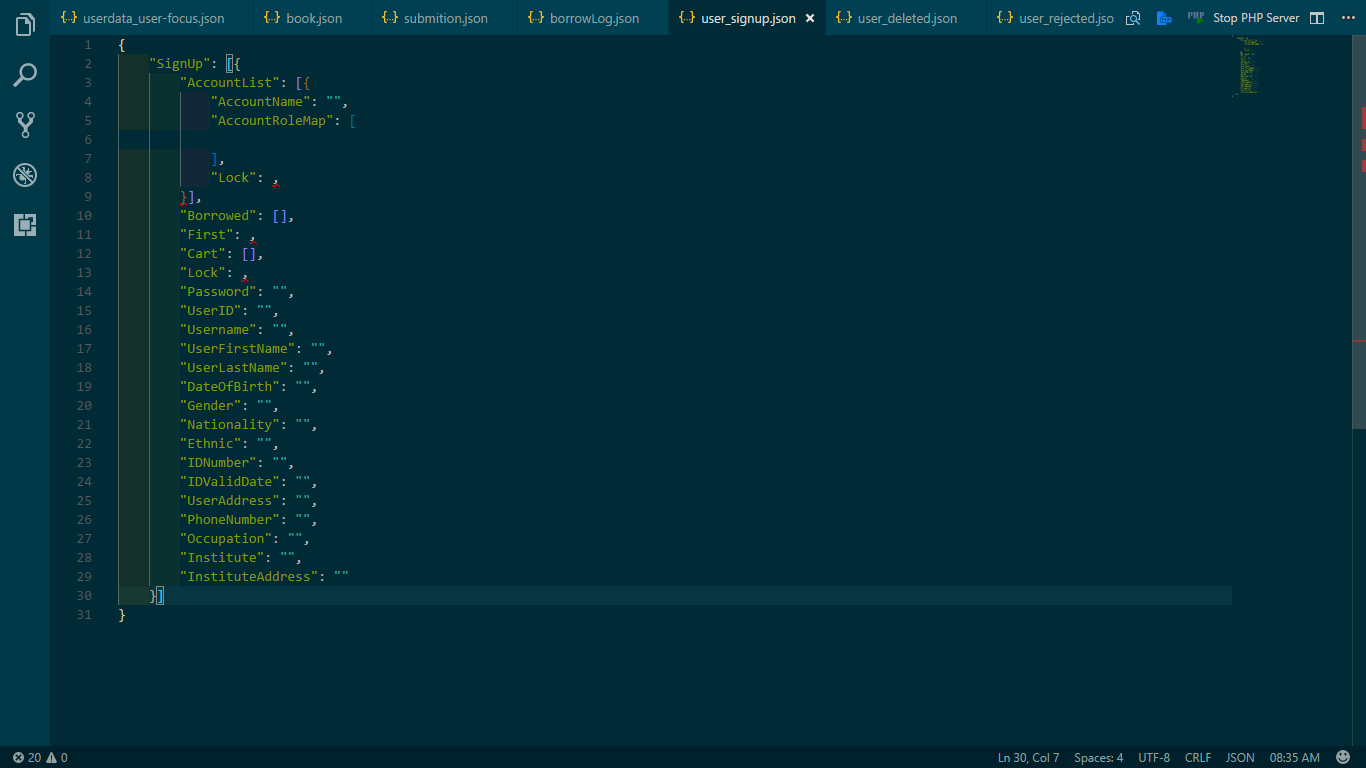
\includegraphics[scale = .3]{user_signup.png}
%                \caption{Sơ đồ các thuộc tính quản lý việc đăng ký}
%            \end{figure}
            \begin{verbatim}
            {
                "SignUp": [
                    {
                        "AccountList": [
                            {
                                "AccountName": string,
                                "AccountRoleMap": [
                                    numbers
                                ],
                                "Lock": true
                            }
                        ],
                        "Balance": number double,
                        "DateOfBirth": string,
                        "Ethnic":string,
                        "First": true,
                        "Gender":string,
                        "IDNumber": string,
                        "IDValidDate": string,
                        "Institue": string,
                        "InstitueAddress": string,
                        "Nationality": string,
                        "Occupation": string,
                        "Password": string,
                        "PhoneNumber": string,
                        "UserAddress": string,
                        "UserFirstName": string,
                        "UserID": string,
                        "UserLastName": string,
                        "Username": string
                    }
                ]
            }
            \end{verbatim}
            \newpage
            \item Tập tin quản lý việc đăng ký không thành công
%            \begin{figure}[H]
%                \centering
%
%                \label{F:user_reject}
%                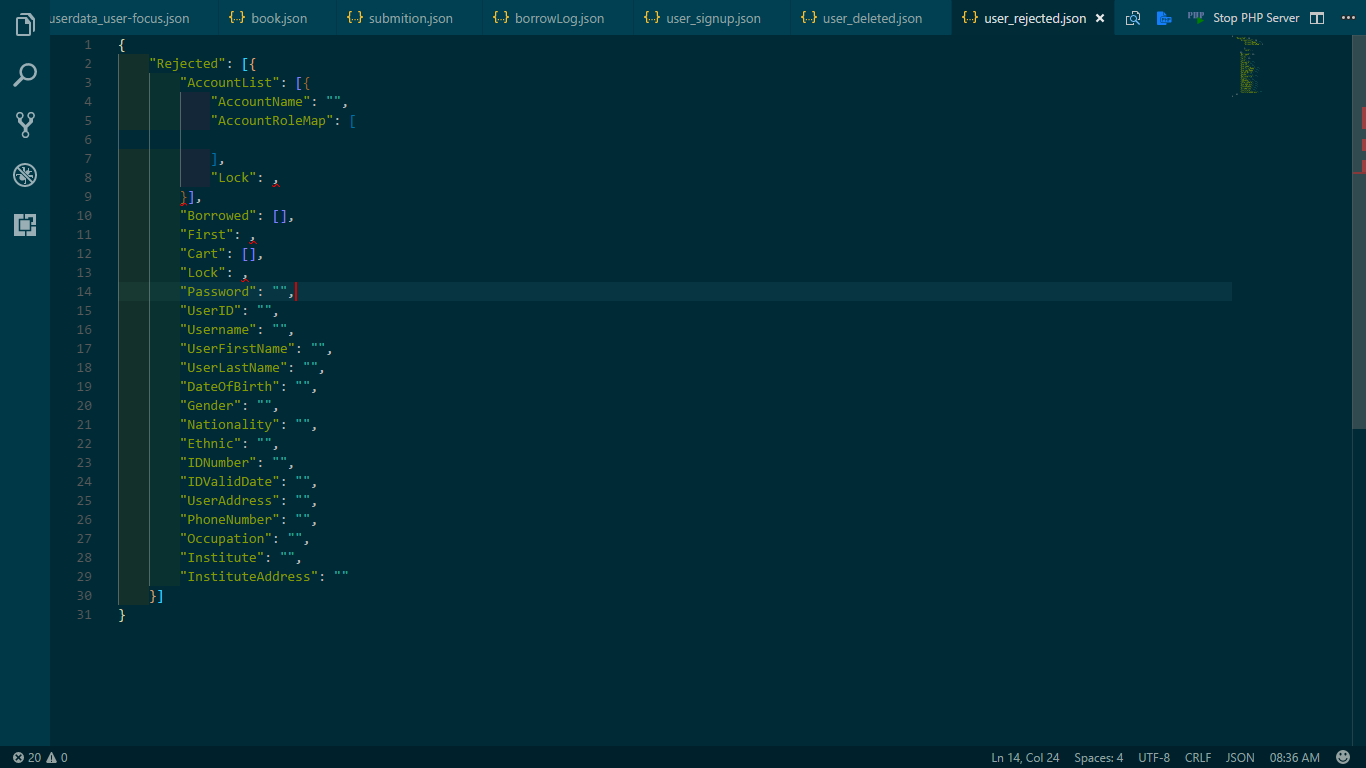
\includegraphics[scale = .3]{user_rejected.png}
%                \caption{Sơ đồ các thuộc tính quản lý việc đăng ký không thành công}
%            \end{figure}
            \begin{verbatim}
            {
                "Rejected": [
                    {
                        "AccountList": [
                            {
                                "AccountName": string,
                                "AccountRoleMap": [
                                    numbers
                                ],
                                "Lock": true
                            }
                        ],
                        "Balance": number double,
                        "DateOfBirth": string,
                        "Ethnic":string,
                        "First": true,
                        "Gender":string,
                        "IDNumber": string,
                        "IDValidDate": string,
                        "Institue": string,
                        "InstitueAddress": string,
                        "Nationality": string,
                        "Occupation": string,
                        "Password": string,
                        "PhoneNumber": string,
                        "UserAddress": string,
                        "UserFirstName": string,
                        "UserID": string,
                        "UserLastName": string,
                        "Username": string
                    }
                ]
            }
            \end{verbatim}
            \newpage
            \item Tập tin quản lý việc xóa người dùng
%            \begin{figure}[H]
%                \centering
%
%                \label{F:userdelete}
%                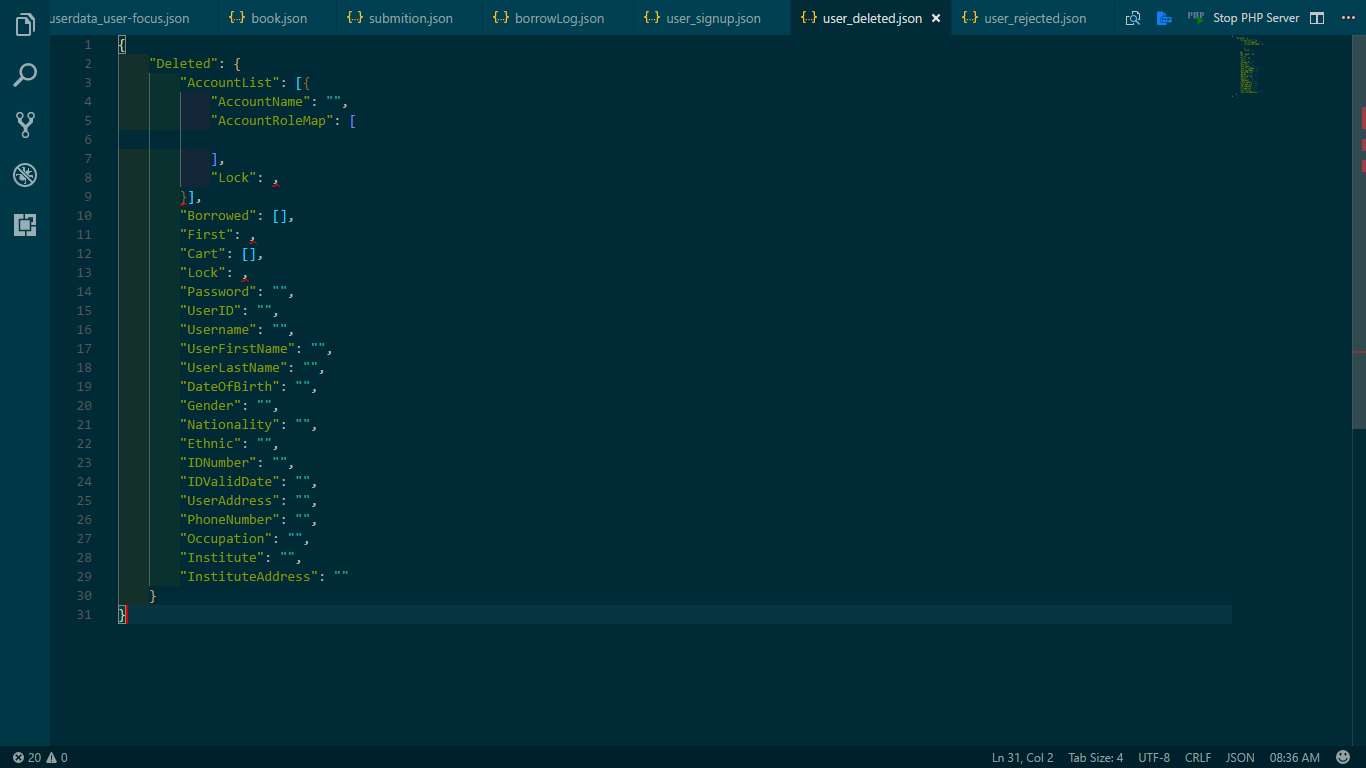
\includegraphics[scale = .3]{user_deleted.png}
%                \caption{Sơ đồ các thuộc tính quản lý việc xóa người dùng}
%            \end{figure}
            \begin{verbatim}
            {
                "Deleted": [
                    {
                        "AccountList": [
                            {
                                "AccountName": string,
                                "AccountRoleMap": [
                                    numbers
                                ],
                                "Lock": true
                            }
                        ],
                        "Balance": number double,
                        "DateOfBirth": string,
                        "Ethnic":string,
                        "First": true,
                        "Gender":string,
                        "IDNumber": string,
                        "IDValidDate": string,
                        "Institue": string,
                        "InstitueAddress": string,
                        "Nationality": string,
                        "Occupation": string,
                        "Password": string,
                        "PhoneNumber": string,
                        "UserAddress": string,
                        "UserFirstName": string,
                        "UserID": string,
                        "UserLastName": string,
                        "Username": string
                    }
                ]
            }
            \end{verbatim}
        \end{enumerate}
        \newpage
        \subsection{Sơ đồ quản lý sách}
        Các sách trong thư viện sẽ được lưu trữ trong cùng một tập tin có sơ đồ như sau:
%            \begin{figure}[H]
%                \centering
%
%                \label{F:book}
%                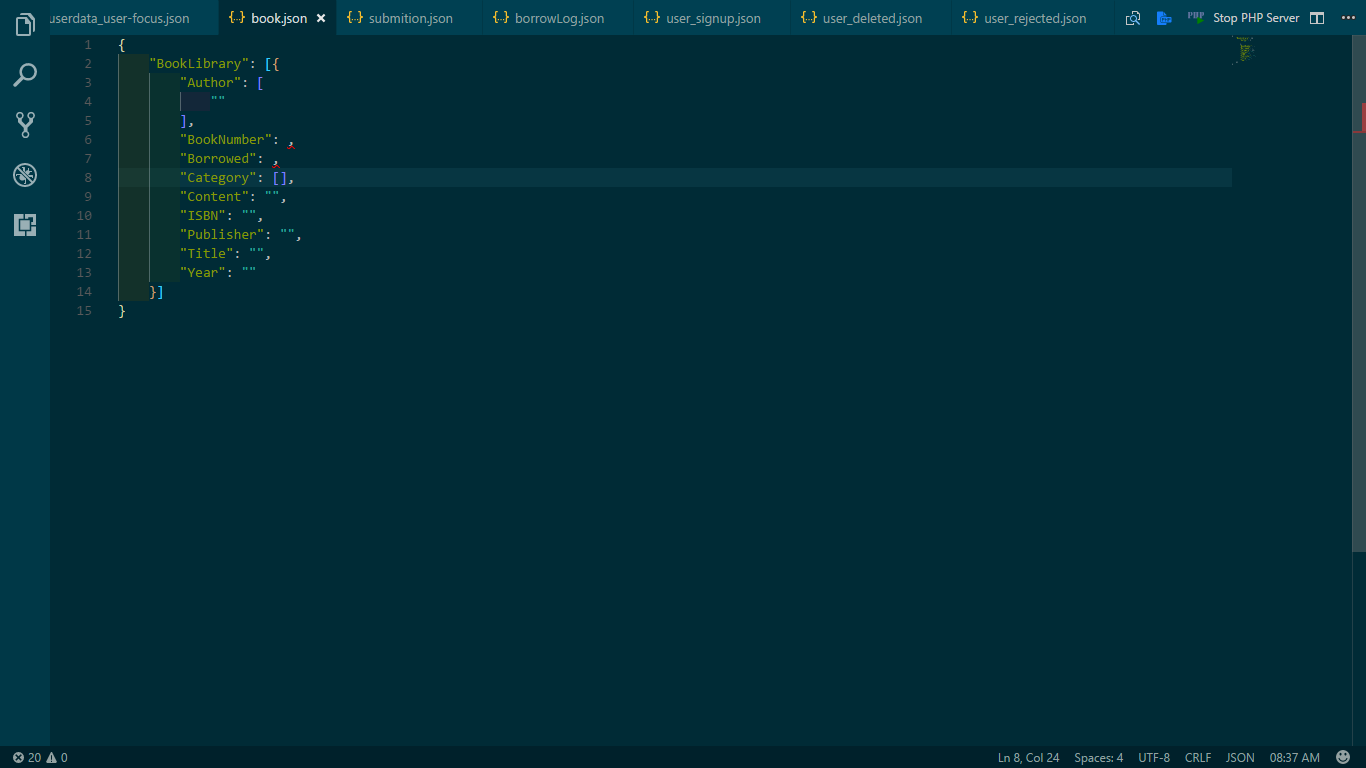
\includegraphics[scale = .3]{book.png}
%                \caption{Sơ đồ các thuộc tính quản lý sách}
%            \end{figure}
        \begin{verbatim}
        {
            "BookLibrary": [
                {
                    "Author": [
                        strings
                    ],
                    "BookNumber": number,
                    "Borrowed": number,
                    "Category": [
                        strings
                    ],
                    "Content": string,
                    "ISBN": string,
                    "Publisher": string,
                    "Title": string,
                    "Year": string
                }
            ]
        }
        \end{verbatim}
        \newpage
        \subsection{Sơ đồ quản lý việc mượn sách}
        Việc lưu trữ các hoạt động mượn trả sách được lưu thành 2 tập tin, có sơ đồ như sau:
            \begin{enumerate}
                \item Tập tin quản lý duyệt mượn sách
%                \begin{figure}[H]
%                \centering
%
%                \label{F:submition}
%                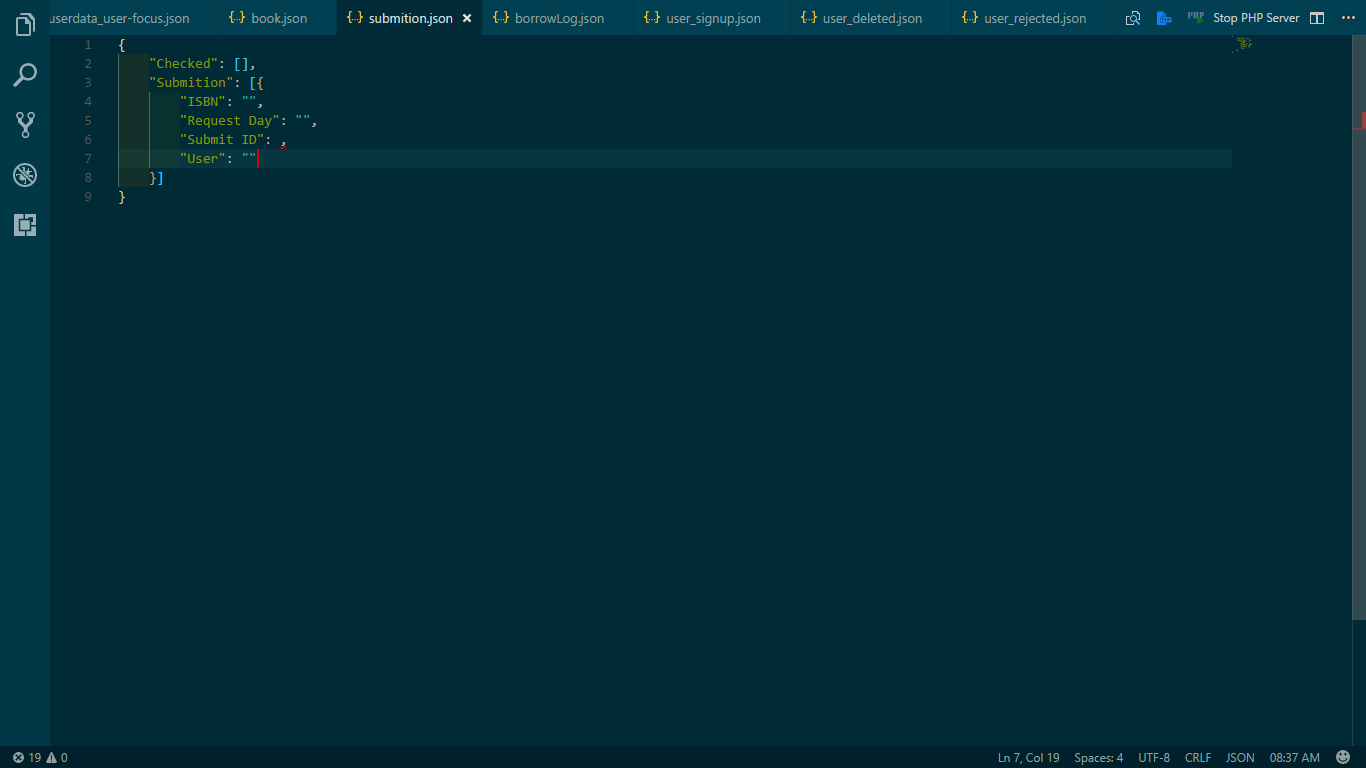
\includegraphics[scale = .3]{submition.png}
%                \caption{Sơ đồ các thuộc tính quản lý duyệt mượn sách}
%            \end{figure}
            \begin{verbatim}
            {
                "Checked": [
                    {
                        "ISBN": string,
                        "Request Date": string,
                        "Submit ID": number,
                        "User": string
                    }
                ],
                "Submission": [
                    {
                        "ISBN": string,
                        "Request Date": string,
                        "Submit ID": number,
                        "User": string
                    }
                ]
            }
            \end{verbatim}
                \newpage
                \item Tập tin quản lý mượn trả sách
%                \begin{figure}[H]
%                \centering
%
%                \label{F:borrowLog}
%                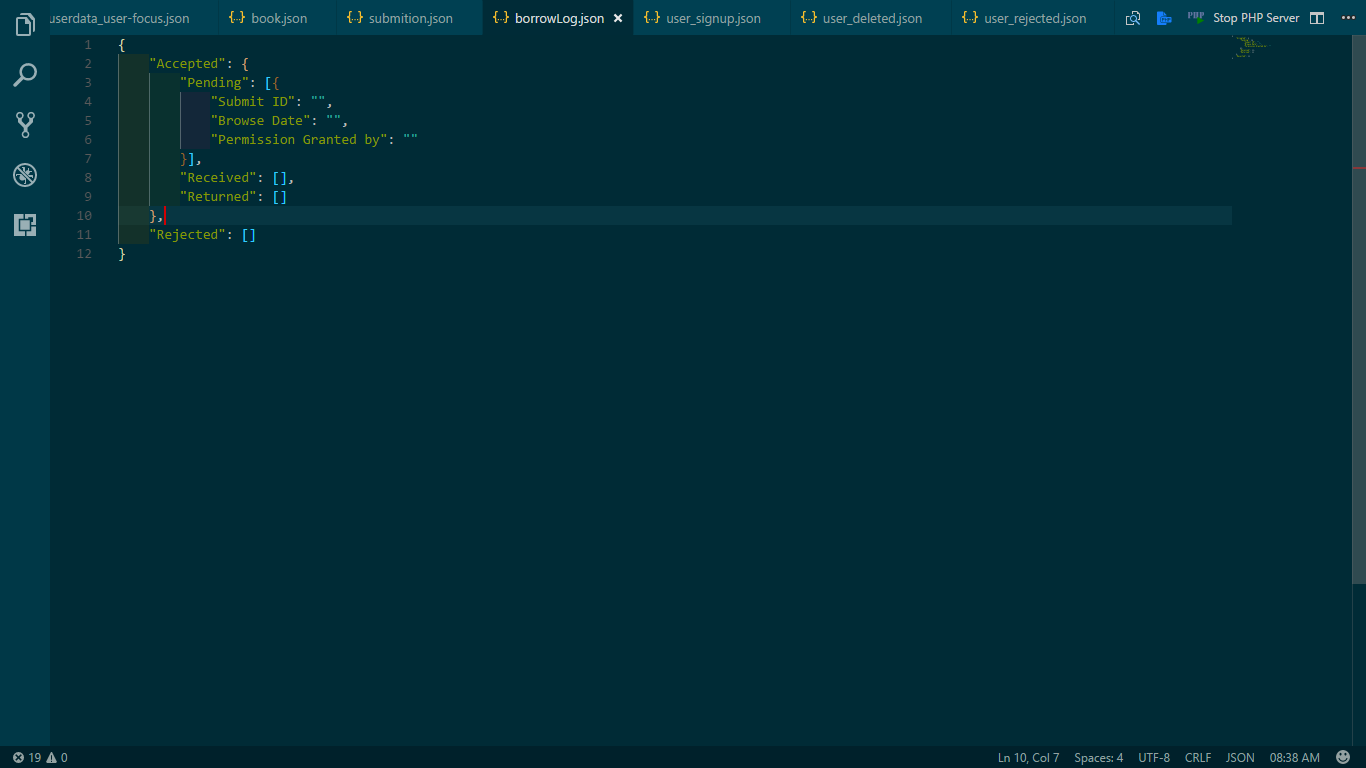
\includegraphics[scale = .3]{borrowlog.png}
%                \caption{Sơ đồ các thuộc tính quản lý mượn trả sách}
%            \end{figure}
            \begin{verbatim}
            {
                "Accepted": {
                    "Pending": [
                        {
                            "Browsed Date": string,
                            "Permission Granted by": string,
                            "Submit ID": number
                        }
                    ],
                    "Received": [
                        {
                            "Browsed Date": string,
                            "Permission Granted by": string,
                            "Received Date": string,
                            "Submit ID": number
                        }
                    ],
                    "Returned": [
                        {
                            "Browsed Date": string,
                            "Permission Granted by": string,
                            "Received Date": string,
                            "Returned Date": string,
                            "Submit ID": number
                        }
                    ]
                }
                "Rejected": [
                    {
                        "Browsed Date": string,
                        "Permission Granted by": string,
                        "Submit ID": number
                    }
                ]
            }
            \end{verbatim}
            \end{enumerate}
    \newpage
    \section{Quá trình làm việc}
        \subsection{Tạo thư mục làm việc trên visualstudio.com}

        Visual Studio gần đây vừa triển khai một ứng dụng mới, và Visual Studio Team Service, giúp các lập trình viên làm việc nhóm chung với nhau thông qua mô hình Agile. Để bắt đầu, bạn cần có một tài khoản của Microsoft, sau đó truy cập theo link sau \url{https://www.visualstudio.com/team-services/} và chọn "Get started for free" để tạo một tên miền của mình. Tên miền sẽ có dạng \url{https://tên miền.visualstudio.com}.\par
        Một tên miền có thể có nhiều dự án (project) và một dự án thì có thể có nhiều nguồn (repository hay repo). Mặc định chúng ta sẽ có một dự án là My Project. Bỏ qua nó và vào trang chủ chọn New Project. Lúc này bạn sẽ có các lựa chọn về tên đự án, chỉ dẫn cho dự án và mô hình làm việc và các phương thức quản lý phiên bản (version control). Về mô hình làm việc, nhóm không biết nhiều về các mô hình này, nên để mặc định là Agile. Về quản lý phiên bản, nhóm thống nhất dùng Git.\par
        Sau khi đã tạo xong, một màn hình yêu cầu upload code lên theo git hiện ra. Sau khi upload code lên, thì chúng ta xem như đã hiện thực xong bước đầu của việc tạo dự án trên Visual Studio Team Service.

        \subsection{Sử dụng Git để quản lý và cập nhật tài liệu}
            \subsubsection{Sơ lược về Git}
        Tổng quan sơ vê Git. Git được hình thành từ khá lâu, bắt nguồn từ những vấn đề với những phần mềm quản lý phiên bản trước đó khi hướng theo code mà không hướng theo tài liệu. Lâu dần, Git được phát triển để từ nay thành một trong những phần mềm quản lý phiên bản được nhiều người sử dụng nhất. \par
        Để bắt đầu với Git, bạn cần lên trang \url{https://git-scm.com/downloads} và tải về Git. Sau khi cài đặt, Git đã ở trên PATH trong máy, bạn có thể hiện thực các câu lệnh trên Git ở trên chính Shell, hoặc sử dụng Git Bash hoặc Git GUI, là những công cụ hỗ trợ riêng của Git. Ở đây nhóm không sử dụng Git GUI, nên thao tác hiện thực là trên Shell.\par

            \subsubsection{Git cơ bản}

            Cùng điểm qua các câu lệnh cơ bản của Git.\\
            Để thực hiện sao lưu thay đổi trong một thư mục (kích hoạt git) thì sẽ sử dụng câu lệnh:
            \begin{verbatim}
                git init
            \end{verbatim}
            Lúc này thư mục sẽ được git quan sát các thay đổi.
            Để lấy về một thư mục đã có, ta có hai cách:
            \begin{verbatim}
                1: git remote add <tên ngắn> <link>
                2: git clone <link>
            \end{verbatim}
            Với clone, tên ngắn được mặc định là origin.
            Trước khi upload, chúng ta phải kiểm tra cho máy cập nhật mới nhất với repo.
            \begin{verbatim}
                git fetch
            \end{verbatim}
            Để lấy về cập nhật và sau đó là
            \begin{verbatim}
                git merge
            \end{verbatim}
            Để ghép các thay đổi vào, xung đội sẽ được đề cập sau.
            Hoặc dùng câu lệnh
            \begin{verbatim}
                git pull
            \end{verbatim}
            Là một hiện thực của hai câu lệnh trên.
            Sau khi đã có code, ta thực hiện thay đôi, git sẽ tự nhận biết thay đổi. Để biết chúng ta đã thay đổi gì,
            \begin{verbatim}
                git status
            \end{verbatim}
            sẽ hiện ra các file chưa được stage, hoặc đã stage nhưng chưa commit.
            Mọi quá trình trên Git đều diễn ra qua 3 giai đoạn,
            \begin{verbatim}
                Stage -> Commit -> (Fetch -> Merge -> Xung đột -> Xử lý) ->Push
            \end{verbatim}
            Stage là để git biết rằng nó sẽ lưu file vào. Commit là để git biết rằng chúng ta muốn lưu lại lúc này, và Push là upload lên repo.
            Khái niệm dùng Git cơ bản khép lại ở đây, và phần nâng cao ngay phía sau.

            \subsubsection{Git nâng cao}
            Khi gặp xung đột lúc merge. Git sẽ yêu cầu xử lý xung đột, và cho chúng ta biết file và chỗ nào trong file. Lúc đó, trên bash sẽ hiện ra tên các file đã xảy ra xung đột, (xung đột thường là khi nhiều người sửa cùng file ở cùng một chỗ, vì cách lưu của Git là theo các bit nên nếu chỗ bit đó bị thay đổi bởi nhiều người thì sẽ nhận biết, ở chỗ khác sẽ không bị xung đột). Chúng ta vô file đó sẽ hiện ra các dòng thế này:\par


            \begin{verbatim}
            <<<<<<< HEAD
            code của ta
            =======
            code trên repo
            >>>>>>> master
            \end{verbatim}
            Có thể không phải là master mà là một chuỗi số, chuỗi số tượng trưng cho lần commit nào đó, hoặc là một nhánh nào đó. Tìm chuỗi đó sẽ cho chúng ta biết được tên của người đã commit lần đó. Từ đó liên hệ với nhau và sửa chỗ đó. Khi sửa xong, chúng ta vẫn push như bình thường.\par

            Tiếp theo là khái niệm cần thiết trong việc làm việc Git. Nhánh. Nhánh (Branch) tương tự như việc khi chúng ta copy code ra USB rồi đưa cho một người khác sửa rồi sau đó ghép lại. Điều tốt hơn việc copy ra USB là khi Git tự động biết được những file nào mà chúng ta đã thay đổi. Đồng thời cho chúng ta xem lại code trước khi ghép lại.\par
            Để bắt đầu tạo nhánh mới, có thể hiện thực trên repo. Hoặc trên Bash:
            \begin{verbatim}
            git checkout -b <tên nhánh mới>
            \end{verbatim}
            Nhánh mới sẽ là một copy của nhánh chúng ta đang ở.
            \begin{verbatim}
            git branch -a
            \end{verbatim}
            Là câu lệnh để biết được tất cả các nhánh, (trước khi hiện thực câu lệnh này, sẽ là một điều khôn ngoan khi lấy dữ liệu từ repo về trước, git fetch). Với dấu sao và màu chữ màu xanh chính là nhánh chúng ta đang ở. Một lưu ý, tạo nhánh trên Bash vẫn chưa được thấy trên repo cho tới khi ta push.\par
            Khi làm việc với nhánh đã xong, chúng ta sẽ bắt đầu ghép vào nhánh gốc hoặc nhánh cha, để thực hiện, chúng ta cần lên repo và tìm pull request. Lúc này sẽ có màn hình về các thông tin đồng thời một danh sách các thanh đổi trong các file để chúng ta xem xét.\par
            Nếu làm việc đơn lẻ, chính chúng ta có thể đồng ý cho duyệt, nhưng khi làm việc nhóm, cần có một Code reviewer, thường là admin, sẽ xem xét code và đưa ra các comment các câu hỏi nếu có thắc mắc trước khi bấm chấp nhận hoặc từ bỏ lần ghép code này.\par
            Git nâng cao còn có nhiều điều nữa nhưng nhóm vẫn chưa thể dùng hết được. Một phần không thuộc Git nhưng lại là một tính tăng quan trọng trong việc lập trình theo một nhóm. Công nghệ tích hợp tự động, Continuous Integration.

            \subsection{Continuous Integration}

            Tích hợp tự động là khi có một sự thay đổi ở nhánh thì sẽ lập tức build, hoặc tích vào đối với ứng dụng web. Nhóm đã thực hiện được trên Visual Studio Team Service và build các lần push lên gần đây. Lợi thế của công cụ này là có thể biết được lỗi xảy ra khi nào và do ai push lên. Đồng thời, tạo một tag để lưu code tại thời điểm đó để có thể quay về. \par

            Điều đầu tiên cần làm là phải biết cách build trên máy của ta. Sau đó hiện thực lại công thức đó trên các máy host hoặc cài một agent về máy xem như là host. Lúc này ta chỉ việc tạo công thức và nếu đúng, với mỗi lần chạy thì sẽ có thể tự động build và tự động tạo tag để ta quản lý.\par

            Sau đây là một ví dụ. Có thể xem thêm thông tin chi tiết tại: \url{https://www.visualstudio.com/team-services/continuous-integration/}\par

            Ví dụ:
        \subsection{Hiện thực phần mềm trên CommandPrompt}
            \subsubsection{Bắt đầu thực hiện và thiết kế}
            Khi nhận được tin báo dự án, cả nhóm đã lên lịch họp và đã bắt đầu code các phần cửa sổ. Vào lúc này, do không có kiến thức nên việc compile được thực hiện một cách không đúng đắn khi include các file cpp vào để khi chạy
            \begin{verbatim}
            g++ -Wall -std=c++11 -c main.cpp -o LIBPRO.exe
            \end{verbatim}
            Thì có thể ra được file chạy hoàn chỉnh.\par

            Sau nhiều ngày nghiên cứu, đã tìm được cách include đúng và compile đúng. Nhưng từ đó lại mở ra một vấn đề khác khi không thể từng tay chạy g++ ra các file o rồi link lại với nhau. Từ đó nhóm ngừng lại trong việc code và tiếp tục nghiên cứu thêm.
            \subsubsection{Phân chia thư mục}
            Cùng lúc đó, nhóm cũng học cách phân chia thư mục, nhận thấy trên mạng có hai cách để phân chia:
            \begin{verbatim}
            include
            src
            và
            project
                module A
                    src
                    include
                module B
                    src
                    include
            \end{verbatim}
            Và quyêt định chọn theo cách ở trên. Vì nhóm chưa có kiến thức và kinh nghiệm trong việc code theo module.
            \subsubsection{Sử dụng JSON cho dữ liệu}
            Ban đầu với việc đọc dữ liệu từ file nhóm vẫn hiện thực rất tốt, nhưng khi tới vấn đề rằng sử dụng các file txt để lưu dữ liệu, một là tạo một hàm chức năng để hiện thực cách lấy dữ liệu trong file; lựa chọn hai là với mỗi file, tạo một hàm mới cho việc đọc và ghi file.\par
            Với cả hai cách, không cách nào là dễ dàng và ngược lại khó nhận dạng thông tin để chỉnh sửa bằng tay. Từ đó, nhóm quyết định sử dụng một loại dữ liệu khác. \par
            Sau khi tìm hiểu, nhóm rút lại các cách gồm có:
            \begin{enumerate}
                \item SQL
                \item MongoDB (do thấy nhiều trên mạng)
                \item thuần JSON
            \end{enumerate}
            Với SQL và MongoDB, học cách để liên kết với dữ liệu trở nên khó khăn và về sau có thể cản trở. Vì thế nhóm quyết định tìm một thư viện để parse JSON nhanh và dễ sử dụng.\par
            Sau khi tìm kiếm, một số cái tên được đưa vào sự chú ý như Rapid JSON, JSON CPP, và đặc biệt nhất là Nlohmann JSON, với cấu trúc dễ dàng cài đặt nhanh chóng chỉ bằng include một file hpp.\par
            Và nhóm quyết định sử dụng JSON, sau đây là một số câu lệnh để sử dụng cơ bản:
            \begin{verbatim}
            using json = nlohmann::json;
            json A = json::object(); // tạo một json object {}
            json B = json::array(); // tạo một json array []
            \end{verbatim}
            Để tạo một key trong A với giá trị item:
            \begin{verbatim}
            A["key"] = item;

            {
                "key": item
            }
            \end{verbatim}
            Để lấy từ file, câu lệnh dùng như đọc file:
            \begin{verbatim}
            ifstream file(path, ios::in);
            json C  = NULL;
            file >> C;
            và xuất ra:
            file << C.dump(4);
            \end{verbatim}
            Để truy cập vào các phần tử,
            \begin{verbatim}
            D.at("key")
            Và thêm vào [chỉ số] nếu nó là array.
            D.at("key")[0].at("FOO") = bar;

            {
                "key": [
                    "FOO": bar
                ]
            }
            \end{verbatim}

            \subsubsection{Build bằng Makefile}

            Quay lại vấn đề build dự án, nhóm đã tìm được cách thức build dự án nhanh hơn khi dùng makefile. Nhóm đã viết các công thức cho makefile sử dụng g++ và build được dự án bằng việc viết.
            \begin{verbatim}
            make tênfile.o
            để build các file cpp thành o và bỏ vào trong thư mục build.

            make libpro hoặc make
            để link các file trong build lại.
            \end{verbatim}
            Makefile hiện đã lỗi thời và nhóm đã xoá đi, tuy nhiên vẫn còn nằm trong lịch sử dự án trong các lần build thành công với tag từ 18 trở xuống.

            \subsubsection{Tạo dự án bằng CMake}
            Với việc xử lý dự án ở trên nhiều công cụ build khác nhau, Makefile phải được thay đổi. Từ đó nhóm lại đi tìm một hình thức khác để tự động hoá dự án. Và đã tìm được CMake.\par
            CMake là công cụ sinh file project, với nhưng ai dùng GNU, CLANG thì sẽ sinh ra Makefile, với những ai dùng Visual Studio thì sẽ sinh ra file sln cùng các file project khác, và tương tự với CodeBlocks, Eclipse, XCode, hay các IDE và các bộ biên dịch khác. Ở đây, nhóm có thiết lập trước với hai compiler là GNU và MSVC (cho Visual Studio).\par
            Sau một khoảng thời gian tìm hiểu, nhóm đã viết được CMakeLists với mục tiêu là lấy tất cả file trong dự án và tạo ra Makefiles có thể build được dự án tốt nhất. Và cũng đã thử với Visual Studio để tạo được dự án với chia thư mục đúng như thư mục đã chia.\par

            Để bắt đầu tạo dự án và build, theo các bước dưới đây. Giả sử đang ở thư mục gốc của dự án.
            \begin{verbatim}
            mkdir build & cd build
            cmake ..
            make
            ../bin/./LIBPRO
            \end{verbatim}
            Nhóm đã tích hợp unit test vào nên nếu muốn build để test:
            \begin{verbatim}
            cmake .. -DTEST=ON
            make
            ../bin/./LIBPRO_TEST
            \end{verbatim}

            \subsubsection{Build cho Linux}

            Với tính năng hỗ trợ Bash cho Windows 10, Linux Subsystem for Windows 10, nhóm đã nghiên cứu để tiến hành build trên Linux. Tuy có gặp một vài trở ngại trong việc sử dụng thư viện, nhưng vẫn có thể build được chương trình cho Unix.
        \subsection{Thiết kế giao diện trên Qt GUI}
            \subsubsection{Thiết kế màn hình chính}
            Màn hình chính được thiết kế đơn giản với thanh menu gồm các nút: Profile-Announcement-Library-Settings-Role-Help.\\
            Khu vực bên dưới thanh menu sẽ trình bày các sách có trong thư viện.\\
            Các chức năng khác được thực hiện trên các cửa sổ con.\\
            \subsubsection{Thiết kế phần cửa sổ con}
            Mỗi cửa sổ con thực hiện một chức nằng nhất định, và có các nút tương ứng với chức năng đó.\\
        %\subsection{Đóng gói phần mềm}
    \section{Thực hiện báo cáo về phần mềm}
        Bản báo cáo này được thực hiện trong suốt quá trình phát triển phần mềm, nhằm cập nhật liên tục các ý tưởng của nhóm. Bản báo cáo cùng với phần báo cáo trên trực tiếp sẽ khái quát rõ hơn về phần mềm của nhóm.
    \section{Lập tài liệu phát triển phần mềm}
        \subsection{Tổ chức dự án}
        SIMple được triển khai thành 2 mảng: CommandPrompt và Qt
            \subsubsection{CommandPrompt}
            \begin{itemize}
                \item bin: chứa các tập tin dữ liệu
                \item include: chứa các file header
                \item libs: chứa thư viện của test
                \item src: chứa các file cpp
                \item test: chứa các file test
                \item .clang-format: đồng bộ code giữa các thành viên
                \item .gitignore: tránh update những tập tin tạm
                \item CMakeList.txt: tập tin chuyên biệt để sử dụng CMake biên dịch chương trình
                \item cppcheck.log: tập tin kiểm tra sai sót cơ bản trong code
                \item folder$\_$structure: tập tin ghi lại cây thư mục của dự án
                \item LIBPRO$\_$ICON.png: tập tin hình ảnh chứa icon của chương trình
                \item README.md: tập tin hướng dẫn sử dụng chương trình
                \item README$\_$INSTALL.md: tập tin hướng dẫn build và cài đặt chương trình
                \item thanhvien.txt: tập tin ghi lại thông tin người phát triển chương trình
            \end{itemize}
            \begin{figure}[H]
                \centering

                \label{F:commandfolder}
                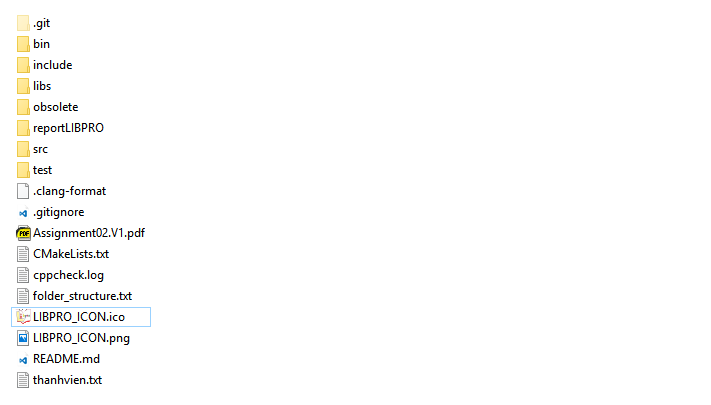
\includegraphics[scale = 1]{commandfolder.png}
                \caption{Các thư mục làm việc của CommandPrompt}
            \end{figure}
            \subsection{Qt GUI}
            Vì đặc điểm phân vùng tập tin trên Qt, các tập tin trong thư mục làm việc trên Qt đều được lưu trên cùng một thư mục
            \begin{itemize}
                \item user$\_$focus: chứa các thư mục làm việc trên CommandPrompt, và đã có một sô chỉnh sửa sao cho phù hợp với Qt GUI (như đã nêu ở trên)
                \item Tập tin new.pro là tập tin gốc để thực thi trên Qt
                \item Tập tin libpro$\_$resource.qrc là tập tin để thêm biểu tượng (icon) cho phần mềm
                \item Còn lại là các tập tin header và source (.h và .cpp)
            \end{itemize}
            \begin{figure}[H]
                \centering

                \label{F:qtfolder}
                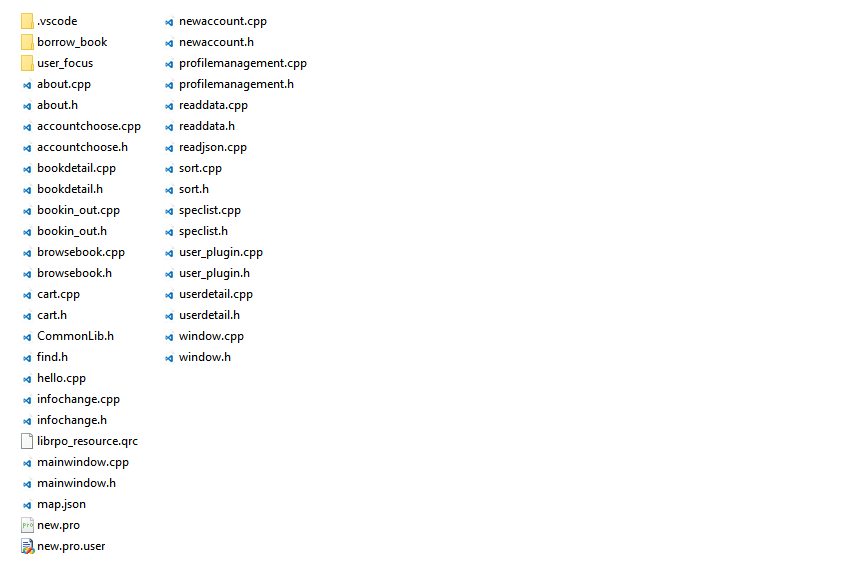
\includegraphics[scale = 1]{qtfolder.png}
                \caption{Các thư mục trong thư mục làm việc Qt}
            \end{figure}
            Trong quá trình biên dịch sẽ tạo ra thư mục mới là \textbf{$build-new-Desktop\_Qt\_5\_8\_0\_MinGW\_32bit-Release$}, trong đó chứa:
            \begin{itemize}
                \item debug: chứa các tập tin link (.o) và các tập tin moc(meta-object compiler) dùng để liên kết với các phần mở rộng của Qt trong quá trình sửa lỗi
                \item release: chứa các tập tin link (.o) và các tập tin moc(meta-object compiler) dùng để liên kết với các phần mở rộng của Qt trong quá trình thực thi
                \item .qmake.stash: ghi lại path các bộ qmake compiler
                \item Makefile: tập tin được tạo ra từ qmake trong quá trình biên dịch
                \item object$\_$script.new.Debug ghi lại các tập tin liên kết (.o) khi chọn cách biên dịch Debug
                \item object$\_$script.new.Release ghi lại các tập tin liên kết (.o) khi chọn cách biên dịch Release
            \end{itemize}
            \begin{figure}[H]
                \centering

                \label{F:buildfolder}
                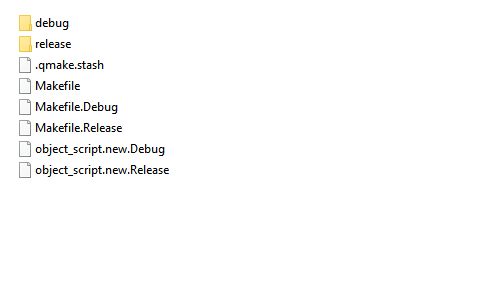
\includegraphics[scale = 1]{buildfolder.png}
                \caption{Các thư mục trong thư mục thực thi Qt}
            \end{figure}
        SIMple thực hiện đồng bộ cả hai mặt nên nhiều hàm trong Qt được thi triển từ các hàm trong CommandPrompt và sử dụng các tập tin header trong CommandPrompt.\\
        \subsection{Thư viện hỗ trợ}
            \subsubsection{Qt GUI}
            Hướng dẫn cài đặt:
            \begin{enumerate}
                \item Vào trang web của Qt và chọn:
                \begin{figure}[H]
                    \centering
                    \label{F:qtstep0}
                    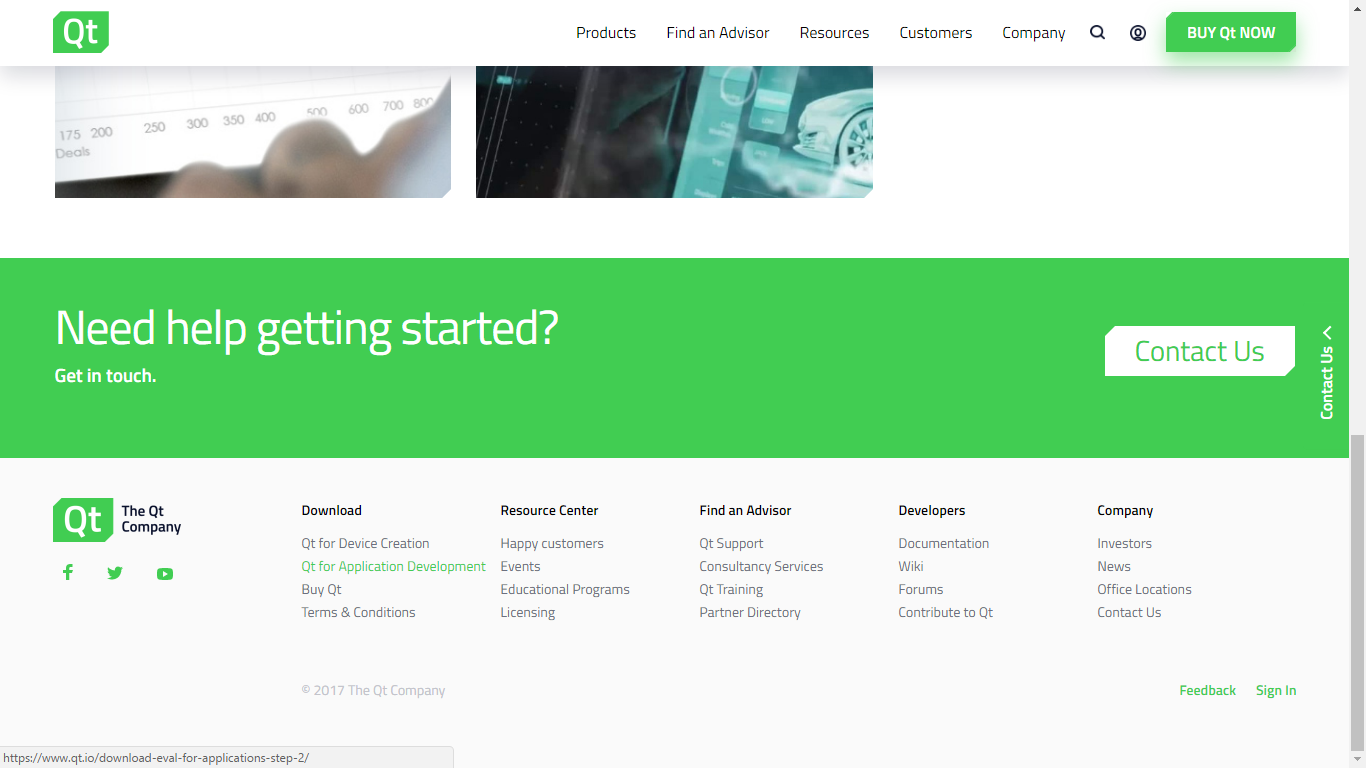
\includegraphics[scale = .3]{Qtstep0.png}
                \end{figure}
                \item Sau đó, chọn ô bên phải, Open Source để tải bản miến phí
                \begin{figure}[H]
                    \centering
                    \label{F:qtstep1}
                    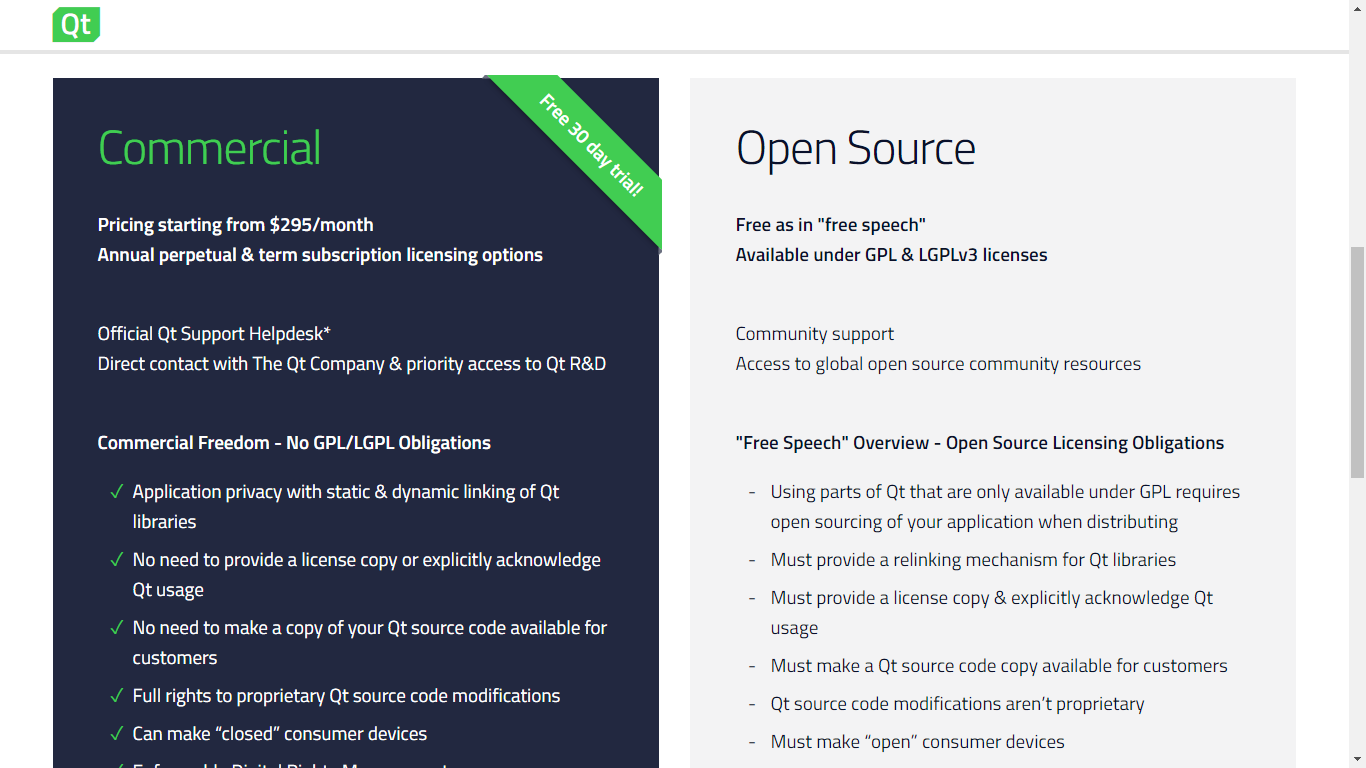
\includegraphics[scale = .3]{Qtstep1.png}
                \end{figure}
                \item Nhập nút Download và Qt sẽ hỏi thư mục muốn tải về, chọn thư mục và OK
                \begin{figure}[H]
                    \centering
                    \label{F:qtstep2}
                    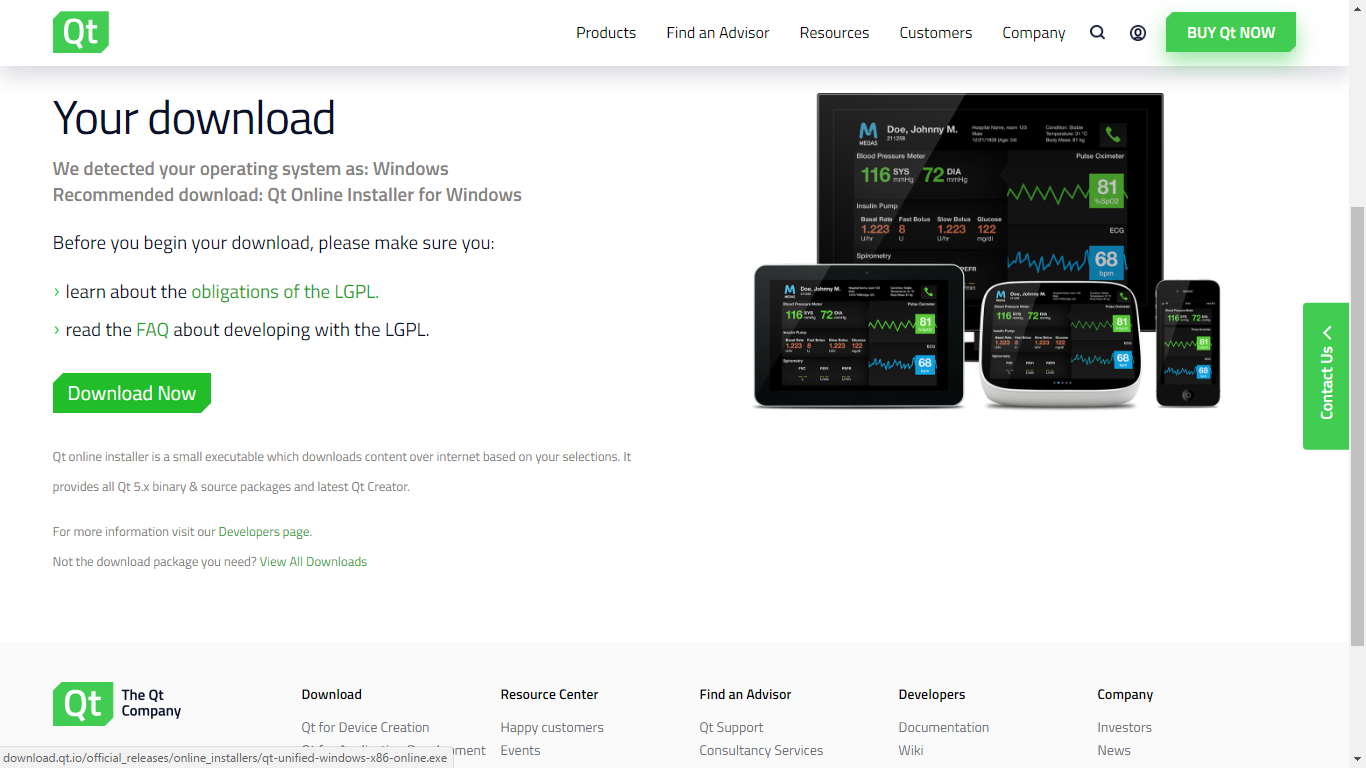
\includegraphics[scale = .3]{Qtstep2.png}
                \end{figure}
                \item Sau khi tải về sẽ có tập tin như thê này
                \begin{figure}[H]
                    \centering
                    \label{F:qtstep3}
                    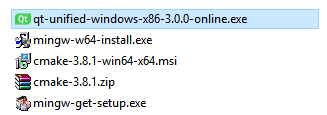
\includegraphics[scale = 2]{Qtstep3.png}
                \end{figure}
                \item Nhấp vào tập tin, sẽ hiện ra cửa sổ như bên dưới, chọn Next
                \begin{figure}[H]
                    \centering
                    \label{F:qtstep4}
                    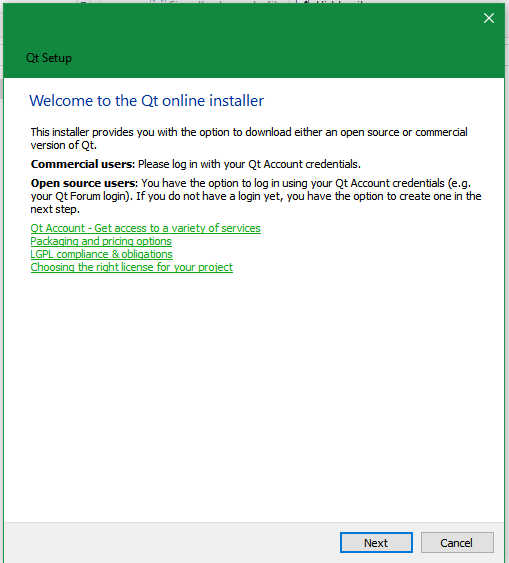
\includegraphics[scale = .7]{Qtstep4.png}
                \end{figure}
                \item Bây giờ, Qt muốn người dùng phải có tài khoản trước khi cài đặt, chọn Login nếu đã có tài khoản hoặc Sign-up nêu chưa có tài khoản
                \begin{figure}[H]
                    \centering
                    \label{F:qtstep5}
                    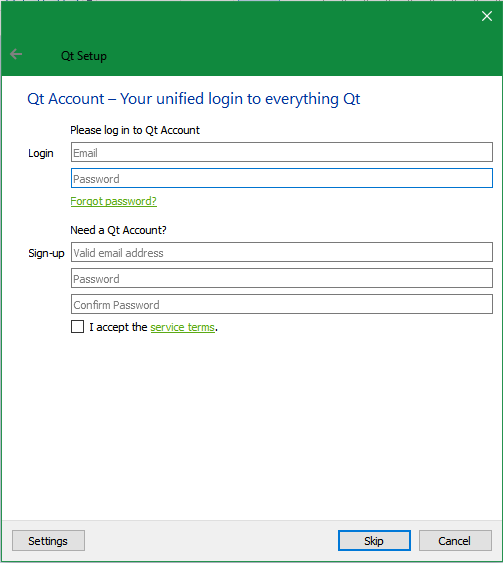
\includegraphics[scale = .7]{Qtstep5.png}
                \end{figure}
                \item Sau khi đã đăng nhập tài khoản, giờ tới cửa sổ Setup, chọn Next để cài đặt
                \begin{figure}[H]
                    \centering
                    \label{F:qtstep6}
                    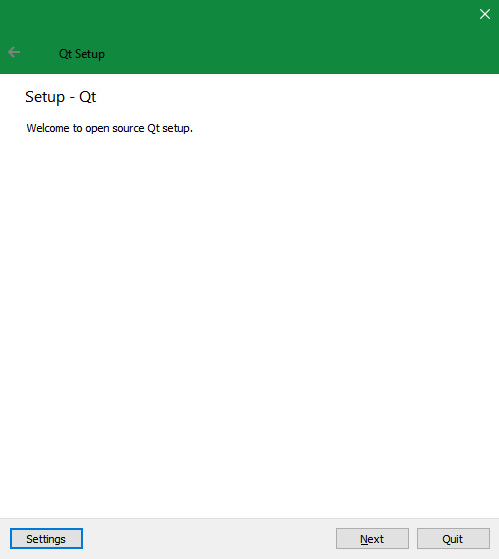
\includegraphics[scale = .7]{Qtstep6.png}
                \end{figure}
                \item Phần cài đặt có thể kéo dài vài giờ đồng hồ, nên người dùng có thể tranh thủ làm việc khác
                \item Sau khi cài đặt xong, tại màn hình Windows, nhấn \textbf{Start->Qt} và chọn \textbf{Qt Creator 4.3.0 (Community)} (có thể tùy theo phiên bản Qt). Đây là môi trường để người dùng thực hiện lập trình giao diện.
                \begin{figure}[H]
                    \centering
                    \label{F:qtstep7}
                    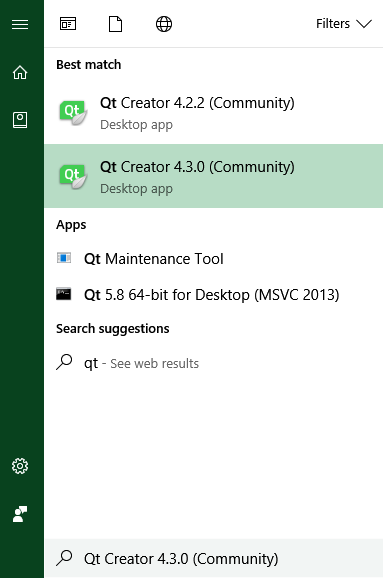
\includegraphics[scale = .7]{Qtstep7.png}
                \end{figure}
            \end{enumerate}
            \subsubsection{GTest}
            Khi nói đến Unit Test trong C++, nhiều người có thể nghĩ tới assert.h. Nhưng nhóm đã không sử dụng thư viện mặc định đó, mà đã sử dung Google Test hay còn gọi tắt là GTest. GTest được Google phát triển và để tự do sử dụng khi để Github public với repo \url{https://github.com/google/googletest}. Để dùng, vào thư mục google test, chạy CMakeLists để ra makefile và chạy tiếp makefile, kết quả cho chúng ta 2 file .a, là file thư viện tĩnh, chúng ta chỉ việc link thư viện vào để sử dụng.\par
            Và để tiện cho việc sử dụng trên chương trình, ta tạo một symbols là UNITTEST, và chính lại hàm main. Vì mọi hàm unit test đều phải được chạy trên một hàm main riêng và sử dụng các định nghĩa hàm trong dự án. Việc còn lại là tạo các hàm test và để trong thư mục test/src và link vào khi chạy CMakeLists với các định nghĩa IF (TEST) và dùng chức năng option(TEST OFF).
        \subsection{Biên dịch và chạy chương trình}
        \subsubsection{Đối với CommandPrompt}
            Để biên dịch chương trình của nhóm, yêu cầu:
            \begin{enumerate}
                \item Một bộ biên dịch hỗ trợ c++11,
                \item Hoặc g++ phiên bản 4.9 trở lên (vì thư viện nlohmann::json yêu cầu)
                \item CMake phiên bản 3.8 trở lên (nếu sử dụng build cho Visual Studio, khuyến khích 3.8.1, vì nhóm đã thực hiện trên phiên bản này để build và thành công)
                \item Nếu sủ dụng Visual Studio, yêu cầu Visual Studio 2013 trở lên, vì sủ dụng chức năng của C++11, phiên bản Visual Studio 2010 không thể build, build hoàn hảo trên Visual Studio 2017, các phiên bản còn lại chưa thử.
            \end{enumerate}
            Đầu tiên là chạy cmake trên một folder mới để sinh ra các file cần thiết để chạy.\par
            Nếu như là biên dịch theo g++ thì chạy makefile, nếu biên dịch theo Visual Studio thì chạy file sln.\par
            Với Visual Studio, cần thực hiện chọn Set as start up project với dự án đang làm để khi build chạy được.\par
        \subsubsection{Đối với Qt Creator}
            sử dụng Build của IDE để thực hiện việc biên dịch.
        \newpage
        \subsection{Hiện thực các hàm chính yếu}
            \subsubsection{Đăng ký và Đăng nhập}
            \begin{enumerate}
                \item Đăng nhập
                \begin{verbatim}
                BEGIN
                Load data
                Choose SignIn
                Enter username and password
                IF (username or password empty)
                    do nothing and return
                ENDIF
                IF (the data is empty)
                    display to user that there is no data
                ENDIF
                IF (username is wrong)
                    display cannot sign in
                ENDIF
                IF (password is wrong)
                    display cannot sign in
                ENDIF
                Get user info as current user
                Display Signed In
                END
                \end{verbatim}
                \newpage
                \item Đăng ký
                \begin{verbatim}
                BEGIN
                Load Data
                Choose Sign Up
                Enter username
                WHILE username exists
                    display message
                    input another username
                ENDWHILE
                Input normal info
                Prompt advanced info
                IF Yes
                    Show advanced info
                ENDIF
                Choose Account package
                IF default
                    Account name = username
                    Package = reader
                ELSE 
                    input account name
                    Choose package
                    IF package = VIP
                        create account with all package
                    ENDIF
                ENDIF
                Generate random password
                Show for user to take note
                IF wrong 
                    END
                ELSE 
                    Send Request
                ENDIF

                Librarian Login
                Browse SignUp
                IF accept
                    move data to user
                ELSE 
                    move data to rejected
                END
                \end{verbatim}
            \end{enumerate}
            \newpage
            \subsubsection{Quản lý xuất nhập sách}
            \begin{enumerate}
                \item Nhập sách mới
                \begin{verbatim}
                BEGIN
                Load data
                User Signed In as Librarian
                Choose add new book
                Input ISBN
                IF (ISBN is a book in data)
                    Ask if add in storage
                    IF true
                        Book number + add in quantity
                    ENDIF
                ENDIF
                Input info of new book
                Update Book Data
                END
            \end{verbatim}
                \item Bỏ sách, xuất sách
                (đây là lựa chọn bỏ hoàn toàn một đầu sách)
                \begin{verbatim}
                BEGIN
                Load data
                User Signed In as Librarian
                Choose Delete book
                Input ISBN
                IF ISBN is not exist
                    require ISBN
                ENDIF
                Input export place
                Change Book number to 0
                Copy book to deleted
                Add export place to book data
                Add date export to book data
                Update book data
                END
                \end{verbatim}
            \end{enumerate}
            \newpage
            \subsubsection{Quản lý mượn trả sách}
                \textbf{Function: BrowseBorrowBook}
                \begin{figure}[H]
                    \centering
                    \label{F:browsebook}
                    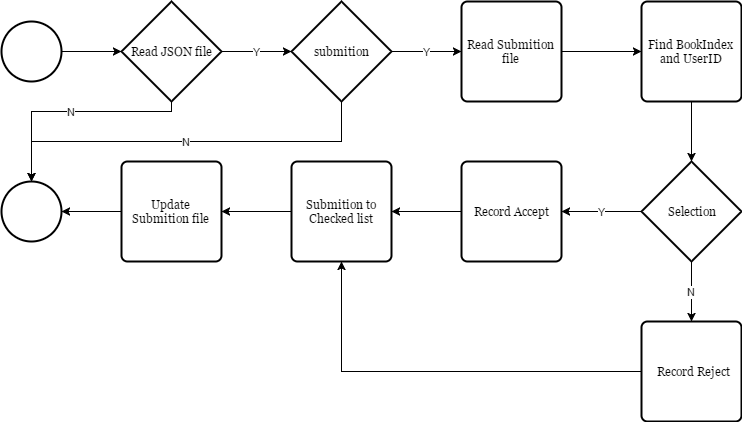
\includegraphics[scale = .4]{browsebook.png}
                    \caption{Sơ đồ khối hoạt động của hàm BrowseBorrowBook}
                \end{figure}
                \begin{verbatim}
                if(!Read JSON file) escape;
                if(!there is submition) escape;
                else{
                    Read Submitions in Submition file;
                    Find BookIndex and UserID in specific Submition;
                    Show selection{
                        if(Accept){
                                Record accepting new submition 
                                to pending place in BorrowLog file;
                        }
                        else Record accepting new submition 
                        to rejected place in BorrowLog file;
                    }
                    Move browsed submition to checked list in Submition file;
                    Update Submition file;
                }
                \end{verbatim}
                \newpage
                \textbf{Function: GiveBook}
                \begin{figure}[H]
                    \centering
                    \label{G:givebook}
                    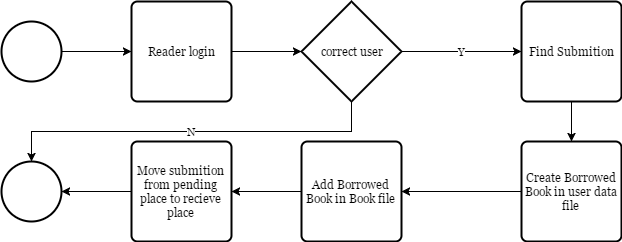
\includegraphics[scale = .4]{givebook.png}
                    \caption{Sơ đồ hoạt động hàm GiveBook}
                \end{figure}
                \begin{verbatim}
                Reader login before getting book (username and password);
                if (correct User Submit){
                        Find Submition of that Reader;
                        Create Borrowed Book in Reader user profile;
                        Add Borrowed Book in Book Library file;
                        Move submititon from pending place to receive place;
                }else escape;
                \end{verbatim}
            \newpage
            \subsubsection{Quản lý hồ sơ người dùng}
                \textbf{Function: VerifyNewUser}
                \begin{figure}[H]
                    \centering
                    \label{F:adduser}
                    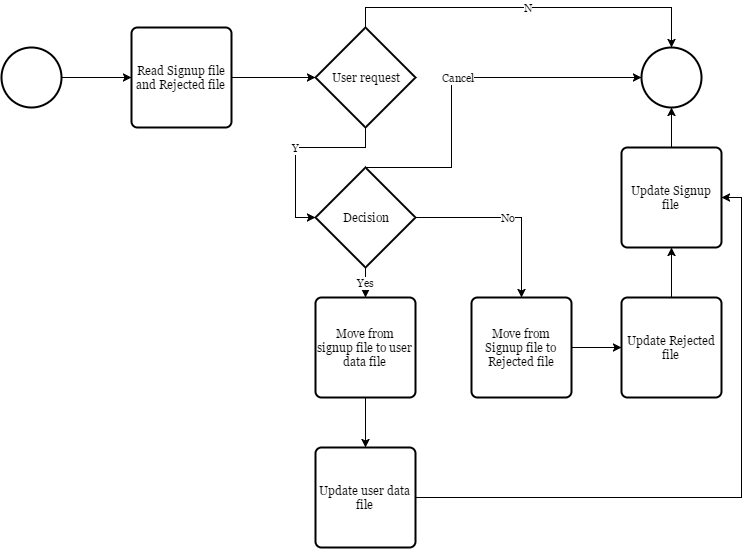
\includegraphics[scale = .4]{adduser.png}
                    \caption{Sơ đồ hoạt động hàm VerifyNewUser}
                \end{figure}
                \begin{verbatim}
                Read Sign-up file and user-rejected file;
                if (no user request) escape;
                else{
                        if (user request decision is Cancel){
                        escape;
                        }
                        else if (user request decision is Yes){
                            Move user profile from sign-up file to user data file;
                            update new user in user data file;
                        }
                        else if(user request decision is No){
                            Move user profile from sign-up file to user-rejected file;
                            update new user in user-rejected file;
                        }
                }
                update signup file;
                \end{verbatim}
                \newpage
                \textbf{Function: DeleteUser}
                \begin{figure}[H]
                    \centering
                    \label{F:deleteuser}
                    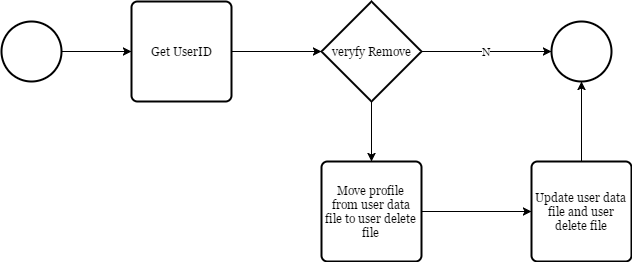
\includegraphics[scale = .4]{deleteuser.png}
                    \caption{Sơ đồ hoạt động hàm DeleteUser}
                \end{figure}
                \begin{verbatim}
                Get UserID to remove;
                if (verifyRemove is No) escape;
                else{
                    Move user profile from user data file to user deleted file;
                    update user data file and user deleted file;
                }
                \end{verbatim}
\chapter{Các vấn đề nảy sinh trong tiến trình phát triển phần mềm}
    \section{Lưu dữ liệu người dùng bằng file *.txt là một trở ngại}
    Trong quá trình làm việc và lưu dữ liệu, nhận thấy việc lưu dữ liệu trong file .txt rất khó truy cập và quản lý, cũng như rất khó hiểu cho người phát triển để kiểm tra dữ liệu. Cụ thể: nếu dữ liệu lưu như thế này:
        \begin{figure}[H]
            \centering
            \label{F:booktext}
            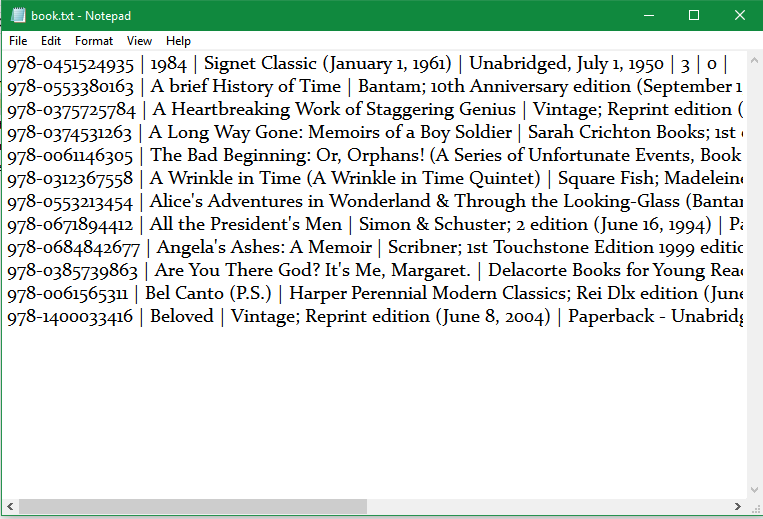
\includegraphics[scale = .7]{booktext.png}
        \end{figure}
    Rõ ràng dù chỉ là dữ liệu sách nhưng lưu với .txt thì không thể nào hiểu được đâu là tên sách, đâu là nhà xuất bản, đâu là tên tác giả. Nên nhất thiết phải có cách lưu dữ liệu hữu hiệu hơn.\\
    \section{Việc đồng bộ hóa giữa dữ liệu và giao diện}
    Vì nhóm chủ yếu tập trung vào thiết kế dữ liệu, nên phần giao diện không thực sự là thế mạnh. Phần mềm chỉ mới được hiện thực các chức năng cơ bản, còn các tính năng mở rộng chỉ mới là ý tưởng.
\end{document}